%%%%%%%%%%%%%%%%%%%%%%%%%%%%%%%%%%%%%%%%%
% The Legrand Orange Book
% Structural Definitions File
% Version 2.0 (9/2/15)
%
% Original author:
% Mathias Legrand (legrand.mathias@gmail.com) with modifications by:
% Vel (vel@latextemplates.com)
% 
% This file has been downloaded from:
% http://www.LaTeXTemplates.com
%
% License:tit
% CC BY-NC-SA 3.0 (http://creativecommons.org/licenses/by-nc-sa/3.0/)
%
%%%%%%%%%%%%%%%%%%%%%%%%%%%%%%%%%%%%%%%%%

%---------------------t-------------------------------------------------------------------
%	VARIOUS REQUIRED PACKAGES AND CONFIGURATIONS
%----------------------------------------------------------------------------------------

\usepackage[top=3cm,bottom=3cm,left=3cm,right=3cm,headsep=10pt,a4paper]{geometry} % Page margins

%\usepackage{graphicx} % Required for including pictures
\usepackage{graphicx} % Required for including pictures
\graphicspath{{Pictures/}} % Specifies the directory where pictures are stored

%\usepackage{lipsum} % Inserts dummy text

%\usepackage{tikz} % Required for drawing custom shapes

\usepackage[english]{babel} % English language/hyphenation

\usepackage{enumitem} % Customize lists
\setlist{nolistsep} % Reduce spacing between bullet points and numbered lists

%\usepackage{booktabs} % Required for nicer horizontal rules in tables

%\usepackage{tcolorbox}
%%% The LaTeX package tcolorbox - version 3.60 (2015/05/07)
%% tcolorbox.sty: Text color boxes
%%
%% -------------------------------------------------------------------------------------------
%% Copyright (c) 2006-2014 by Prof. Dr. Dr. Thomas F. Sturm <thomas dot sturm at unibw dot de>
%% -------------------------------------------------------------------------------------------
%%
%% This work may be distributed and/or modified under the
%% conditions of the LaTeX Project Public License, either version 1.3
%% of this license or (at your option) any later version.
%% The latest version of this license is in
%%   http://www.latex-project.org/lppl.txt
%% and version 1.3 or later is part of all distributions of LaTeX
%% version 2005/12/01 or later.
%%
%% This work has the LPPL maintenance status `author-maintained'.
%%
%% This work consists of all files listed in README
%%
\NeedsTeXFormat{LaTeX2e}
%\ProvidesPackage{tcolorbox}[2015/05/07 version 3.60 text color boxes]
%\def\tcb@version{3.60}

\RequirePackage{pgf}[2008/01/15]
\RequirePackage{verbatim}[2003/08/22]
%\input{environ.sty}
%\RequirePackage{environ}[2013/04/01]
\RequirePackage{etoolbox}[2011/01/03]

% register
\newif\iftcb@lowerignored
\newif\iftcb@lowervisible
\newif\iftcb@uppervisible
\newif\iftcb@hasTitle
\newif\iftcb@hasLower
\newif\iftcb@lowerspace
\newif\iftcb@sidebyside
\newif\iftcb@hasPhantom
\newif\iftcb@lowerseparated
\newif\iftcb@titlefilled
\newif\iftcb@fixedheight
\newif\iftcb@ignorenobreak

\newbox\tcb@titlebox
\newbox\tcb@upperbox
\newbox\tcb@lowerbox
\newbox\tcb@phantombox

\newcounter{tcbbreakpart}
\newcounter{tcblayer}

\def\tcb@warning#1{\PackageWarning{tcolorbox}{#1}}
\def\tcb@error#1#2{\PackageError{tcolorbox}{#1}{#2}}

% key management
\pgfkeys{/tcb/.is family}

\def\tcbset{\pgfqkeys{/tcb}}
\long\def\tcbset@late@options#1{\appto\tcb@lateoptions@hook{\tcbset{#1}}}

\def\tcb@dim@to#1#2{\def#1{\the\dimexpr#2\relax}}
\def\tcbdimto#1#2{\edef#1{\the\dimexpr#2\relax}}

\def\tcb@defToTotalHeightStandard#1#2{\tcbdimto#1{\ht#2+\dp#2}}
\let\tcb@defToTotalHeight\tcb@defToTotalHeightStandard

\def\tcb@zpt{0pt}

\def\tcb@comp@arc@auto{%
  \let\tcb@outer@arc=\kvtcb@top@rule@stand%
  \ifdim\kvtcb@bottom@rule@stand<\tcb@outer@arc\relax%
    \let\tcb@outer@arc=\kvtcb@bottom@rule@stand\fi%
  \ifdim\kvtcb@left@rule<\tcb@outer@arc\relax%
    \let\tcb@outer@arc=\kvtcb@left@rule\fi%
  \ifdim\kvtcb@right@rule<\tcb@outer@arc\relax%
    \let\tcb@outer@arc=\kvtcb@right@rule\fi%
  \tcbdimto\tcb@outer@arc{\tcb@arc@scale\dimexpr\tcb@outer@arc\relax+\kvtcb@arc}%
}

\def\tcb@comp@arc@fix{%
  \tcbdimto\tcb@outer@arc{\kvtcb@outerarc}%
}

\def\tcb@use@auto@parskip{%
  \tcbset{autoparskip}%
}

\def\tcb@hack@currenvir{\edef\tcb@temp{\noexpand\def\noexpand\@currenvir{\kvtcb@savedelimiter}}\tcb@temp}

\def\tcb@sbs@quota@leftwidth{%
  \tcbdimto\tcb@w@upper{\kvtcb@sbs@ratio}%
  \tcbdimto\tcb@w@lower{\tcb@w@sbs-\tcb@w@upper}%
}

\def\tcb@sbs@quota@rightwidth{%
  \tcbdimto\tcb@w@lower{\kvtcb@sbs@ratio}%
  \tcbdimto\tcb@w@upper{\tcb@w@sbs-\tcb@w@lower}%
}

\def\tcb@sbs@quota@leftratio{%
  \tcbdimto\tcb@w@upper{\kvtcb@sbs@ratio\dimexpr\tcb@w@sbs}%
  \tcbdimto\tcb@w@lower{\tcb@w@sbs-\tcb@w@upper}%
}

\def\tcb@sbs@quota@rightratio{%
  \tcbdimto\tcb@w@lower{\kvtcb@sbs@ratio\dimexpr\tcb@w@sbs}%
  \tcbdimto\tcb@w@upper{\tcb@w@sbs-\tcb@w@lower}%
}

\def\tcb@shield@@externalize{%
  \ifdefined\tikzexternaldisable%
    \ifdefined\pgfpictureid%
    \else%
      \tikzexternaldisable%
    \fi%
  \fi}

\def\tcb@set@embed@tcbox#1{%
  \long\def\tcb@embed@tcbox##1{%
    \tcbdimto\tcb@w@upper{\kvtcb@width-\kvtcb@left@rule-\kvtcb@leftupper-\kvtcb@boxsep*2-\kvtcb@rightupper-\kvtcb@right@rule}%
    #1}%
}

\def\tcb@new@skin#1#2{\tcbset{skin@#1/.style={#2}}}
\newcommand{\tcbsubskin}[3]{\tcb@new@skin{#1}{skin@#2,#3}}

\pgfkeys{/handlers/.dimstore in/.code=\pgfkeysalso{\pgfkeyscurrentpath/.code=\def#1{\the\dimexpr##1\relax}}}
\pgfkeys{/handlers/.colorlet/.code=\pgfkeysalso{\pgfkeyscurrentpath/.code=\colorlet{#1}{##1}}}

\newcommand\tcbtitle{\ifx\tcbtitletext\@empty\else%
  {\color{tcbcol@title}\kvtcb@fonttitle\kvtcb@haligntitle\kvtcb@before@title\tcbtitletext\kvtcb@after@title}\fi}

\def\tcb@detach@title@code@{%
  \let\tcbtitletext\kvtcb@title%
  \let\kvtcb@title\@empty%
  \tcbset{title/.store in=\tcbtitletext}%
  \let\tcb@detach@title@code\@empty%
  \let\tcb@attach@title@code\tcb@attach@title@code@%
  \let\tcb@specialtitle@hook\@empty%
}

\def\tcb@attach@title@code@{%
  \let\kvtcb@title\tcbtitletext%
  \let\tcbtitletext\@empty%
  \tcbset{title/.store in=\kvtcb@title}%
  \let\tcb@attach@title@code\@empty%
  \let\tcb@detach@title@code\tcb@detach@title@code@%
  \let\tcb@specialtitle@hook\@empty%
}

% analog to plain.tex
\def\tcb@raggedright@plain{\raggedright\rightskip0pt plus2em \spaceskip.3333em \xspaceskip.5em\relax}
\def\tcb@raggedleft@plain{\raggedleft\leftskip0pt plus2em \spaceskip.3333em \xspaceskip.5em \hbadness=10000\relax}
\def\tcb@raggedcenter@plain{\centering\leftskip0pt plus2em\rightskip0pt plus2em\spaceskip.3333em \xspaceskip.5em \hbadness=10000\relax}

\tcbset{%
  title/.store in=\kvtcb@title,
  notitle/.style={title=},
  adjust text/.store in=\kvtcb@adjusttext,
  adjusted title/.style={title={#1\vphantom{\kvtcb@adjusttext}}},
  squeezed title/.style={title={%
    \setbox\z@=\color@hbox#1\color@endbox%
    \ifdim\wd\z@>\linewidth\relax%
      \resizebox{\linewidth}{\height}{\unhbox\z@}%
    \else%
      \unhbox\z@%
    \fi%
  }},
  squeezed title*/.style={squeezed title={#1\vphantom{\kvtcb@adjusttext}}},%
  detach title/.code=\tcb@detach@title@code,%
  attach title/.code=\tcb@attach@title@code,%
  attach title to upper/.style={detach title,before upper={\tcbtitle#1}},
  attach title to upper/.default=,
  subtitle style/.store in=\kvtcb@subtitle@style,%
  width/.store in=\kvtcb@width,
  text width/.style={width={#1+\kvtcb@left@rule+\kvtcb@right@rule+\kvtcb@boxsep*2+\kvtcb@leftupper+\kvtcb@rightupper}},%
  add to width/.code={\tcbdimto\kvtcb@width{\kvtcb@width+(#1)}},%
  boxsep/.store in=\kvtcb@boxsep,
  toprule/.code={%
    \def\kvtcb@top@rule@stand{#1}%
    \let\kvtcb@top@rule@break=\kvtcb@top@rule@stand%
    },
  bottomrule/.code={%
    \def\kvtcb@bottom@rule@stand{#1}%
    \let\kvtcb@bottom@rule@break=\kvtcb@bottom@rule@stand%
    },
  leftrule/.store in=\kvtcb@left@rule,
  rightrule/.store in=\kvtcb@right@rule,
  titlerule/.store in=\kvtcb@title@rule,
  boxrule/.code={
    \def\kvtcb@top@rule@stand{#1}%
    \let\kvtcb@top@rule@break=\kvtcb@top@rule@stand%
    \let\kvtcb@bottom@rule@stand=\kvtcb@top@rule@stand%
    \let\kvtcb@bottom@rule@break=\kvtcb@top@rule@stand%
    \let\kvtcb@left@rule=\kvtcb@top@rule@stand%
    \let\kvtcb@right@rule=\kvtcb@top@rule@stand%
    \let\kvtcb@title@rule=\kvtcb@top@rule@stand%
    },
  arc/.store in=\kvtcb@arc,
  outer arc/.code={\def\kvtcb@outerarc{#1}\let\tcb@comp@arc=\tcb@comp@arc@fix},
  auto outer arc/.code={\let\tcb@comp@arc=\tcb@comp@arc@auto},
  circular arc/.style={arc=\tcb@innerwidth/2},
  bean arc/.code={%
    \iftcb@fixedheight%
      \ifdim\dimexpr\kvtcb@width-\kvtcb@left@rule-\kvtcb@right@rule>\dimexpr\kvtcb@height@fixed-\kvtcb@top@rule@stand-\kvtcb@bottom@rule@stand\relax%
        \def\kvtcb@arc{(\kvtcb@height@fixed-\kvtcb@top@rule@stand-\kvtcb@bottom@rule@stand)/2}%
      \else%
        \def\kvtcb@arc{(\kvtcb@width-\kvtcb@left@rule-\kvtcb@right@rule)/2}%
      \fi%
    \else%
      \def\kvtcb@arc{\tcb@innerwidth/2}%
    \fi%
  },
  octogon arc/.style={arc=0.292893218\dimexpr\tcb@innerwidth\relax},
  arc is curved/.code={%
    \def\tcb@arc@scale{1}%
    \let\tcb@apply@graph@patches=\tcbpatcharcround%
  },
  arc is angular/.code={%
    \def\tcb@arc@scale{0.58578644}%
    \let\tcb@apply@graph@patches=\tcbpatcharcangular%
  },
  sharpish corners/.style={arc=0pt,outer arc=0pt},
  lefttitle/.store in=\kvtcb@lefttitle,
  leftupper/.store in=\kvtcb@leftupper,
  leftlower/.store in=\kvtcb@leftlower,
  left/.style={lefttitle=#1,leftupper=#1,leftlower=#1},
  righttitle/.store in=\kvtcb@righttitle,
  rightupper/.store in=\kvtcb@rightupper,
  rightlower/.store in=\kvtcb@rightlower,
  right/.style={righttitle=#1,rightupper=#1,rightlower=#1},
  top/.store in=\kvtcb@top,
  toptitle/.store in=\kvtcb@toptitle,
  bottom/.store in=\kvtcb@bottom,
  bottomtitle/.store in=\kvtcb@bottomtitle,
  middle/.store in=\kvtcb@middle,
  colback/.colorlet=tcbcol@back,
  colframe/.colorlet=tcbcol@frame,
  colupper/.colorlet=tcbcol@upper,
  collower/.colorlet=tcbcol@lower,
  coltext/.style={colupper=#1,collower=#1},
  coltitle/.colorlet=tcbcol@title,
  fonttitle/.store in=\kvtcb@fonttitle,
  fontupper/.store in=\kvtcb@fontupper,
  fontlower/.store in=\kvtcb@fontlower,
  tempfile/.store in=\kvtcb@tempfile,
  savelowerto/.store in=\kvtcb@savelowerto,
  saveto/.store in=\kvtcb@saveupperto,
  savedelimiter/.estore in=\kvtcb@savedelimiter,
  floatplacement/.store in=\kvtcb@floatplacement,
  float/.code={\def\kvtcb@float{#1}\def\tcb@float@env@begin{\@float}\def\tcb@float@env@end{\end@float}},
  float/.default=\kvtcb@floatplacement,
  float*/.code={\def\kvtcb@float{#1}\def\tcb@float@env@begin{\@dblfloat}\def\tcb@float@env@end{\end@dblfloat}},
  float*/.default=\kvtcb@floatplacement,
  every float/.store in=\kvtcb@everyfloat,%
  nofloat/.style={float=},
  before/.code={\def\kvtcb@beforebox{#1}\let\tcb@use@autoparskip=\relax},
  after/.code={\def\kvtcb@afterbox{#1}\let\tcb@use@autoparskip=\relax},
  autoparskip/.code={\let\tcb@use@autoparskip=\tcb@use@auto@parskip},
  parskip/.style={before={\par\pagebreak[0]\parindent=0pt},after={\par}},
  noparskip/.style={before={\ifnum\lastnodetype=-1\relax\else\par\smallskip\pagebreak[0]\fi\parindent=0pt},after={\par\smallskip}},
  nobeforeafter/.style={before=,after=},
  force nobeforeafter/.code={\tcbset@late@options{nobeforeafter}},
  before skip/.style={before={%
    \ifnum\lastnodetype=-1\relax%
    \else%
      \par\ifvmode\nointerlineskip%
      \addvspace{\glueexpr#1-\parskip}%
      \fi%
    \fi%
    \lineskip=0pt\noindent%
    }},
  after skip/.style={after={%
    \par\ifvmode\nointerlineskip%
    \addvspace{\glueexpr#1-\parskip}\fi%
    }},
  beforeafter skip/.style={before skip={#1},after skip={#1}},
  before nobreak/.store in=\kvtcb@beforebox@nobreak,
  lowerbox/.is choice,
  lowerbox/visible/.code={\tcb@lowerignoredfalse\tcb@lowervisibletrue},
  lowerbox/invisible/.code={\tcb@lowerignoredfalse\tcb@lowervisiblefalse},
  lowerbox/ignored/.code={\tcb@lowerignoredtrue\tcb@lowervisiblefalse},
  upperbox/.is choice,
  upperbox/visible/.code={\tcb@uppervisibletrue},
  upperbox/invisible/.code={\tcb@uppervisiblefalse},
  visible/.style={upperbox=visible,lowerbox=visible},
  invisible/.style={upperbox=invisible,lowerbox=invisible},
  natural height/.code={\tcb@fixedheightfalse\let\tcb@ch=\tcb@ch@natural\let\tcb@height@adjust\@empty},
  height/.code={\tcb@fixedheighttrue\tcb@dim@to\kvtcb@height@fixed{#1}\let\tcb@ch=\tcb@ch@fixed\let\tcb@height@adjust\@empty},
  text height/.code={\tcb@fixedheighttrue\tcb@dim@to\kvtcb@height@fixed{#1}\let\tcb@ch=\tcb@ch@innerfixed\let\tcb@height@adjust\@empty},
  add to height/.code={\ifdefined\kvtcb@height@fixed\tcbdimto\kvtcb@height@fixed{\kvtcb@height@fixed+(#1)}\fi},
  height plus/.dimstore in=\kvtcb@height@fixed@plus,%
  height from/.style args={#1 to #2}{height={#1},height plus={#2-#1}},%
  height fill/.is choice,%
  height fill/false/.code={\let\tcb@height@adjust\@empty},%
  square/.style={height=\kvtcb@width},
  equal height group/.code={\edef\tcb@ehgid{#1}\let\tcb@ch=\tcb@ch@equalheight},
  minimum for equal height group/.code args={#1:#2}{\edef\tcb@ehgid{#1}\tcb@ehgadd{#2}},
  space/.code={\def\tcb@height@fraction{#1}\let\tcb@ch@fixed@both=\tcb@ch@fixed@space},
  space to upper/.style={space=1},
  space to lower/.style={space=0},
  space to both/.style={space=0.5},
  split/.code={\def\tcb@height@fraction{#1}\let\tcb@ch@fixed@both=\tcb@ch@fixed@split},
  %
  halign/.is choice,
  halign/flush left/.code={\let\kvtcb@halignupper=\raggedright},
  halign/flush right/.code={\let\kvtcb@halignupper=\raggedleft},
  halign/flush center/.code={\let\kvtcb@halignupper=\centering},
  halign/left/.code={\let\kvtcb@halignupper=\tcb@raggedright@plain},
  halign/right/.code={\let\kvtcb@halignupper=\tcb@raggedleft@plain},
  halign/center/.code={\let\kvtcb@halignupper=\tcb@raggedcenter@plain},
  halign/justify/.code={\let\kvtcb@halignupper=\@empty},
  halign upper/.style={halign=#1},
  %
  halign lower/.is choice,
  halign lower/flush left/.code={\let\kvtcb@halignlower=\raggedright},
  halign lower/flush right/.code={\let\kvtcb@halignlower=\raggedleft},
  halign lower/flush center/.code={\let\kvtcb@halignlower=\centering},
  halign lower/left/.code={\let\kvtcb@halignlower=\tcb@raggedright@plain},
  halign lower/right/.code={\let\kvtcb@halignlower=\tcb@raggedleft@plain},
  halign lower/center/.code={\let\kvtcb@halignlower=\tcb@raggedcenter@plain},
  halign lower/justify/.code={\let\kvtcb@halignlower=\@empty},
  %
  halign title/.is choice,
  halign title/flush left/.code={\let\kvtcb@haligntitle=\raggedright},
  halign title/flush right/.code={\let\kvtcb@haligntitle=\raggedleft},
  halign title/flush center/.code={\let\kvtcb@haligntitle=\centering},
  halign title/left/.code={\let\kvtcb@haligntitle=\tcb@raggedright@plain},
  halign title/right/.code={\let\kvtcb@haligntitle=\tcb@raggedleft@plain},
  halign title/center/.code={\let\kvtcb@haligntitle=\tcb@raggedcenter@plain},
  halign title/justify/.code={\let\kvtcb@haligntitle=\@empty},
  %
  valign/.is choice,
  valign/top/.code={\def\kvtcb@valignupper{top}},
  valign/center/.code={\def\kvtcb@valignupper{center}},
  valign/bottom/.code={\def\kvtcb@valignupper{bottom}},
  valign upper/.style={valign=#1},
  valign lower/.is choice,
  valign lower/top/.code={\def\kvtcb@valignlower{top}},
  valign lower/center/.code={\def\kvtcb@valignlower{center}},
  valign lower/bottom/.code={\def\kvtcb@valignlower{bottom}},
  enlarge top initially by/.store in=\kvtcb@bbtop@stand,%
  enlarge top at break by/.store in=\kvtcb@bbtop@break,%
  enlarge top by/.style={enlarge top initially by={#1},enlarge top at break by={#1}},%
  enlarge bottom finally by/.store in=\kvtcb@bbbottom@stand,%
  enlarge bottom at break by/.store in=\kvtcb@bbbottom@break,%
  enlarge bottom by/.style={enlarge bottom finally by={#1},enlarge bottom at break by={#1}},%
  enlarge left by/.store in=\kvtcb@bbleft,
  enlarge right by/.store in=\kvtcb@bbright,
  enlarge by/.style={enlarge top by={#1},enlarge bottom by={#1},enlarge left by={#1},enlarge right by={#1}},%
  grow to left by/.code={%
    \tcbdimto\kvtcb@width{\kvtcb@width+#1}%
    \pgfkeysalso{enlarge left by={-\the\dimexpr#1\relax}}},%
  grow to right by/.code={%
    \tcbdimto\kvtcb@width{\kvtcb@width+#1}%
    \pgfkeysalso{enlarge right by={-\the\dimexpr#1\relax}}},%
  left skip/.style={grow to left by={-#1}},
  right skip/.style={grow to right by={-#1}},
  leftright skip/.style={left skip={#1},right skip={#1}},
  toggle enlargement/.is choice,
  toggle enlargement/none/.code={\let\tcb@setbb@toggle=\tcb@setbb@toggle@none},
  toggle enlargement/evenpage/.code={\let\tcb@setbb@toggle=\tcb@setbb@toggle@evenpage},
  toggle enlargement/forced/.code={\let\tcb@setbb@toggle=\tcb@setbb@toggle@forced},
  toggle enlargement/.default=evenpage,
  toggle left and right/.is choice,
  toggle left and right/none/.code={\let\tcb@lrtoggle=\tcb@lrtoggle@none},
  toggle left and right/evenpage/.code={\let\tcb@lrtoggle=\tcb@lrtoggle@evenpage},
  toggle left and right/forced/.code={\let\tcb@lrtoggle=\tcb@lrtoggle@forced},
  toggle left and right/.default=evenpage,
  graphical environment/.store in=\kvtcb@graphenv,
  %
  frame engine/.is choice,
  frame engine/standard/.style={frame code=\tcb@drawframe@standard},
  frame engine/standardjigsaw/.style={frame code=\tcb@drawframe@standardjigsaw},
  frame code/.code={\def\tcb@frame@code{#1}},%
  frame code/.default=\tcb@drawframe@standard,%
  frame empty/.style={frame code=},
  %
  interior titled engine/.is choice,
  interior titled engine/standard/.style={interior titled code=\tcb@drawwithtitle@standard},
  interior titled code/.code={\def\tcb@interiortitled@code{#1}},%
  interior titled code/.default=\tcb@drawwithtitle@standard,%
  interior titled empty/.style={interior titled code=},
  %
  interior engine/.is choice,
  interior engine/standard/.style={interior code=\tcb@drawwithouttitle@standard},
  interior code/.code={\def\tcb@interior@code{#1}},%
  interior code/.default=\tcb@drawwithouttitle@standard,%
  interior empty/.style={interior code=},
  %
  segmentation engine/.is choice,
  segmentation engine/standard/.style={segmentation code=\tcb@drawlower@standard},
  segmentation code/.code={\def\tcb@segmentation@code{#1}},%
  segmentation code/.default=\tcb@drawlower@standard,%
  segmentation empty/.style={segmentation code=},
  %
  title engine/.is choice,
  title engine/standard/.style={@title code=\tcb@drawtitle@standard},
  @title code/.code={\def\tcb@title@code{#1}},%
  @title code/.default=\tcb@drawtitle@standard,%
  title code/.style={title filled,@title code={#1}},%
  title code/.default=\tcb@drawtitle@standard,%
  title empty/.style={@title code=},
  %
  geometry nodes/.store in=\kvtcv@geonodes,
  geometry nodes/.default=true,%
  set@extensions@preframe/.store in=\tcb@extensions@preframe,%
  set@extensions@postframe/.store in=\tcb@extensions@postframe,%
  set@extensions@final/.store in=\tcb@extensions@final,%
  set@outerboundary/.store in=\tcb@outerboundary,%
  skin first/.store in=\kvtcb@skin@first,
  skin middle/.store in=\kvtcb@skin@middle,
  skin last/.store in=\kvtcb@skin@last,
  skin/.style={skin@#1},
  skin first is subskin of/.style 2 args={skin@local@first/.style={skin@#1,#2},skin first=local@first},%
  skin middle is subskin of/.style 2 args={skin@local@middle/.style={skin@#1,#2},skin middle=local@middle},%
  skin last is subskin of/.style 2 args={skin@local@last/.style={skin@#1,#2},skin last=local@last},%
  parbox/.store in=\kvtcv@parbox,
  parbox/.default=true,%
  hyphenationfix/.is choice,%
  hyphenationfix/.default=true,%
  hyphenationfix/true/.code={\def\tcb@hyph@fix{\everypar=\expandafter{\the\everypar\everypar{\hspace{0pt}}\hspace{0pt}}}},%
  hyphenationfix/false/.code={\let\tcb@hyph@fix=\@empty},%
  overlay unbroken/.code={\def\tcb@overlay@unbroken{#1}},%
  overlay first/.code={\def\tcb@overlay@first{#1}},%
  overlay middle/.code={\def\tcb@overlay@middle{#1}},%
  overlay last/.code={\def\tcb@overlay@last{#1}},%
  overlay/.code={\def\tcb@overlay@temp{#1}%
    \let\tcb@overlay@unbroken=\tcb@overlay@temp%
    \let\tcb@overlay@first=\tcb@overlay@temp%
    \let\tcb@overlay@middle=\tcb@overlay@temp%
    \let\tcb@overlay@last=\tcb@overlay@temp},%
  overlay broken/.code={\def\tcb@overlay@temp{#1}%
    \let\tcb@overlay@first=\tcb@overlay@temp%
    \let\tcb@overlay@middle=\tcb@overlay@temp%
    \let\tcb@overlay@last=\tcb@overlay@temp},%
  overlay unbroken and first/.code={\def\tcb@overlay@temp{#1}%
    \let\tcb@overlay@unbroken=\tcb@overlay@temp%
    \let\tcb@overlay@first=\tcb@overlay@temp},%
  overlay unbroken and last/.code={\def\tcb@overlay@temp{#1}%
    \let\tcb@overlay@unbroken=\tcb@overlay@temp%
    \let\tcb@overlay@last=\tcb@overlay@temp},%
  overlay middle and last/.code={\def\tcb@overlay@temp{#1}%
    \let\tcb@overlay@middle=\tcb@overlay@temp%
    \let\tcb@overlay@last=\tcb@overlay@temp},%
  overlay first and middle/.code={\def\tcb@overlay@temp{#1}%
    \let\tcb@overlay@first=\tcb@overlay@temp%
    \let\tcb@overlay@middle=\tcb@overlay@temp},%
  no overlay/.style={overlay=},%
  standard/.style={skin=standard},%
  standard jigsaw/.style={skin=standard jigsaw},%
  before title/.store in=\kvtcb@before@title,%
  after title/.store in=\kvtcb@after@title,%
  before upper/.store in=\kvtcb@before@upper,%
  after upper/.store in=\kvtcb@after@upper,%
  before lower/.store in=\kvtcb@before@lower,%
  after lower/.store in=\kvtcb@after@lower,%
  center title/.style={halign title=flush center},%
  center upper/.style={halign upper=flush center},%
  center lower/.style={halign lower=flush center},%
  flushleft title/.style={halign title=flush left},%
  flushleft upper/.style={halign upper=flush left},%
  flushleft lower/.style={halign lower=flush left},%
  flushright title/.style={halign title=flush right},%
  flushright upper/.style={halign upper=flush right},%
  flushright lower/.style={halign lower=flush right},%
  tabularx*/.style 2 args={%
    boxsep=0pt,top=0pt,bottom=0pt,leftupper=0pt,rightupper=0pt,
    toptitle=1mm,bottomtitle=1mm,boxrule=0.5mm,
    before upper={\arrayrulecolor{tcbcol@frame}\def\arraystretch{1.1}#1%
      \tcb@hack@currenvir\tabularx{\linewidth}{#2}},
    after upper=\endtabularx\arrayrulecolor{black}},
  tabularx/.style={tabularx*={}{#1}},
  tikz upper/.style={before upper=\centering\tcb@shield@externalize\begin{tikzpicture}[#1],after upper=\end{tikzpicture}},%
  tikz lower/.style={before lower=\centering\tcb@shield@externalize\begin{tikzpicture}[#1],after lower=\end{tikzpicture}},%
  tikznode upper/.style={before upper={\centering\tcb@shield@externalize\begin{tikzpicture}\node[align=center,inner sep=0pt,outer sep=0pt,#1]\bgroup},after upper={\egroup;\end{tikzpicture}}},%
  tikznode lower/.style={before lower={\centering\tcb@shield@externalize\begin{tikzpicture}\node[align=center,inner sep=0pt,outer sep=0pt,#1]\bgroup},after lower={\egroup;\end{tikzpicture}}},%
  tikznode/.style={tikznode upper={#1},tikznode lower={#1}},%
  varwidth upper/.style={before upper={\tcbdimto\tcb@w@upper{#1-\kvtcb@left@rule-\kvtcb@right@rule-\kvtcb@boxsep*2-\kvtcb@leftupper-\kvtcb@rightupper}%
    \begin{varwidth}{\tcb@w@upper}},after upper={\end{varwidth}}},%
  varwidth upper/.default=\kvtcb@width,
  oversize/.style={%
    width=\the\dimexpr\dimexpr\linewidth+#1+\kvtcb@left@rule+\kvtcb@leftupper+\kvtcb@boxsep*2+\kvtcb@rightupper+\kvtcb@right@rule\relax,%
    enlarge left by=\the\dimexpr-\kvtcb@left@rule-\kvtcb@leftupper-\kvtcb@boxsep-#1/2\relax,%
    enlarge right by=\the\dimexpr-\kvtcb@boxsep-\kvtcb@rightupper-\kvtcb@right@rule-#1/2\relax},%
  oversize/.default=0pt,%
  baseline/.store in=\kvtcb@baseline,%
  tcbox raise/.style={baseline=-#1},%
  tcbox raise base/.style={baseline=\tcb@val@raisebase},%
  box align/.is choice,%
  box align/bottom/.style={baseline=0pt},%
  box align/top/.style={baseline=\tcb@height},%
  box align/center/.style={baseline=\tcb@height/2},%
  box align/base/.style={baseline=\tcb@val@raisebase},%
  shrink tight/.style={boxsep=0mm,top=-\kvtcb@top@rule@stand,bottom=-\kvtcb@bottom@rule@stand,left=-\kvtcb@left@rule,right=-\kvtcb@right@rule},%
  extrude left by/.code={\tcbdimto\kvtcb@leftupper{\kvtcb@leftupper+#1}\tcbdimto\kvtcb@bbleft{\kvtcb@bbleft-#1}\tcbdimto\kvtcb@width{\kvtcb@width+#1}},%
  extrude right by/.code={\tcbdimto\kvtcb@rightupper{\kvtcb@rightupper+#1}\tcbdimto\kvtcb@bbright{\kvtcb@bbright-#1}\tcbdimto\kvtcb@width{\kvtcb@width+#1}},%
  extrude top by/.code={\tcbdimto\kvtcb@top{\kvtcb@top+#1}\tcbdimto\kvtcb@bbtop@stand{\kvtcb@bbtop@stand-#1}},%
  extrude bottom by/.code={\tcbdimto\kvtcb@bottom{\kvtcb@bottom+#1}\tcbdimto\kvtcb@bbbottom@stand{\kvtcb@bbbottom@stand-#1}},%
  extrude by/.style={extrude left by=#1,extrude right by=#1,extrude top by=#1,extrude bottom by=#1},%
  sidebyside/.is if=tcb@sidebyside,%
  sidebyside align/.is choice,%
  sidebyside align/top/.code={\def\kvtcb@sbs@align{top}\def\tcb@box@align##1{}},%
  sidebyside align/center/.code={\def\kvtcb@sbs@align{center}\def\tcb@box@align##1{}},%
  sidebyside align/bottom/.code={\def\kvtcb@sbs@align{bottom}\def\tcb@box@align##1{}},%
  sidebyside align/top seam/.code={\def\kvtcb@sbs@align{top}\let\tcb@box@align\tcb@box@align@top},%
  sidebyside align/center seam/.code={\def\kvtcb@sbs@align{center}\let\tcb@box@align\tcb@box@align@center},%
  sidebyside align/bottom seam/.code={\def\kvtcb@sbs@align{bottom}\let\tcb@box@align\tcb@box@align@bottom},%
  sidebyside gap/.dimstore in=\kvtcb@sbs@gap,%
  lefthand width/.code={\def\kvtcb@sbs@ratio{#1}\let\tcb@sbs@quota=\tcb@sbs@quota@leftwidth},
  righthand width/.code={\def\kvtcb@sbs@ratio{#1}\let\tcb@sbs@quota=\tcb@sbs@quota@rightwidth},
  lefthand ratio/.code={\def\kvtcb@sbs@ratio{#1}\let\tcb@sbs@quota=\tcb@sbs@quota@leftratio},
  righthand ratio/.code={\def\kvtcb@sbs@ratio{#1}\let\tcb@sbs@quota=\tcb@sbs@quota@rightratio},
  breakable@false/.code={%
    \let\tcb@savebox=\tcb@lrbox%
    \let\endtcb@savebox=\endtcb@lrbox%
    \let\tcb@defToTotalHeight=\tcb@defToTotalHeightStandard%
    \let\tcb@drawcolorbox=\tcb@drawcolorbox@standalone},
  code/.code={#1},
  capture/.store in=\kvtcb@capture,%
  hbox/.style={capture=hbox},%
  minipage/.style={capture=minipage},%
  check odd page/.is choice,
  check odd page/true/.code={\let\tcb@checkoddpage=\checkoddpage%
    \def\tcb@evenoddmode{strict}%
    },
  check odd page/false/.code={\let\tcb@checkoddpage=\relax%
    \def\tcb@evenoddmode{easy}%
    },
  check odd page/.default=true,
  phantom/.code={\appto\kvtcb@phantom{#1}},
  step and label/.style 2 args={phantom={\refstepcounter{#1}\tcb@set@label{#2}}},%
  step/.style={phantom={\refstepcounter{#1}}},%
  label/.style={phantom={\tcb@set@label{#1}}},%
  phantomlabel/.style={phantom={\ifdefined\phantomsection\phantomsection\fi\tcb@set@label{#1}}},%
  label type/.store in=\kvtcb@label@type,%
  no label type/.style={label type=},%
  add to list/.style 2 args={phantom={\tcb@addcontentsline{#1}{#2}}},
  nophantom/.code={\def\kvtcb@phantom{}},%
  shield externalize/.is choice,
  shield externalize/true/.code={\let\tcb@shield@externalize=\tcb@shield@@externalize},
  shield externalize/false/.code={\let\tcb@shield@externalize=\relax},
  shield externalize/.default=true,
  external/.code={\tikzsetnextfilename{#1}},
  remake/.code={\tikzset{external/remake next={#1}}},
  remake/.default=true,
  lower separated/.is if=tcb@lowerseparated,
  options@for/.code={\letcs\tcb@new@colop{tcb@opt@#1}\pgfkeysalsofrom\tcb@new@colop},
  list entry/.store in=\kvtcb@listentry,
  list text/.style={list entry={\protect\numberline{\thetcbcounter}{\ignorespaces #1}}},
  title filled/.is if=tcb@titlefilled,%
  @colbacktitle/.colorlet=tcbcol@backtitle,
  colbacktitle/.style={title filled,@colbacktitle={#1}},
  opacityupper/.store in=\kvtcb@opacityupper,
  opacitylower/.store in=\kvtcb@opacitylower,
  opacitytitle/.store in=\kvtcb@opacitytitle,
  opacityframe/.store in=\kvtcb@opacityframe,
  opacityback/.store in=\kvtcb@opacityback,
  @opacitybacktitle/.store in=\kvtcb@opacitybacktitle,
  opacitybacktitle/.style={title filled,@opacitybacktitle={#1}},
  opacityfill/.style={opacityframe={#1},opacityback={#1},@opacitybacktitle={#1}},
  opacitytext/.style={opacityupper={#1},opacitylower={#1}},
  spartan@fit/.code={},%
  %
  size/.is choice,
  size/normal/.style={boxrule=0.5mm,boxsep=1mm,left=4mm,right=4mm,top=2mm,bottom=2mm,toptitle=0pt,bottomtitle=0pt,
    middle=2mm,arc=1mm,auto outer arc},
  size/title/.style={boxrule=0.4mm,boxsep=1mm,left=2mm,right=2mm,top=0.25mm,bottom=0.25mm,toptitle=0pt,bottomtitle=0pt,
    middle=0.75mm,arc=0.75mm,auto outer arc},
  size/small/.style={boxrule=0.3mm,boxsep=1mm,left=1mm,right=1mm,top=0pt,bottom=0pt,toptitle=0pt,bottomtitle=0pt,
    middle=0.5mm,arc=0.5mm,auto outer arc},
  size/fbox/.style={boxrule=0.4pt,boxsep=3pt,left=0pt,right=0pt,top=0pt,bottom=0pt,toptitle=0pt,bottomtitle=0pt,
    middle=1pt,arc=1pt,auto outer arc},
  size/tight/.style={boxrule=0.4pt,boxsep=0pt,left=0pt,right=0pt,top=0pt,bottom=0pt,toptitle=0pt,bottomtitle=0pt,
    middle=0.2pt,arc=0pt,outer arc=0pt},
  size/minimal/.style={boxrule=0pt,boxsep=0pt,left=0pt,right=0pt,top=0pt,bottom=0pt,toptitle=0pt,bottomtitle=0pt,
    middle=0pt,arc=0pt,outer arc=0pt},
  on line/.style={tcbox raise base,nobeforeafter},
  shape@of@skin/.store in=\tcb@shapeofskin,
  ignore nobreak/.is if=tcb@ignorenobreak,%
  only/.code args={<#1>#2}{\only<#1>{\tcbset{#2}}},%
  %
  tcbox width/.is choice,
  tcbox width/auto/.code={\def\tcb@embed@tcbox{}},
  tcbox width/auto limited/.code={\tcb@set@embed@tcbox{%
    \setbox\z@=\color@hbox##1\color@endbox\ifdim\wd\z@<\tcb@w@upper\relax\box\z@\else%
    \begin{minipage}{\tcb@w@upper}##1\end{minipage}\fi}},
  tcbox width/forced center/.code={\tcb@set@embed@tcbox{\makebox[\tcb@w@upper]{##1}}},
  tcbox width/forced left/.code={\tcb@set@embed@tcbox{\makebox[\tcb@w@upper][l]{##1}}},
  tcbox width/forced right/.code={\tcb@set@embed@tcbox{\makebox[\tcb@w@upper][r]{##1}}},
  tcbox width/minimum center/.code={\tcb@set@embed@tcbox{%
    \setbox\z@=\color@hbox##1\color@endbox\ifdim\wd\z@<\tcb@w@upper\relax\makebox[\tcb@w@upper]{\box\z@}\else\box\z@\fi}},
  tcbox width/minimum left/.code={\tcb@set@embed@tcbox{%
    \setbox\z@=\color@hbox##1\color@endbox\ifdim\wd\z@<\tcb@w@upper\relax\makebox[\tcb@w@upper][l]{\box\z@}\else\box\z@\fi}},
  tcbox width/minimum right/.code={\tcb@set@embed@tcbox{%
    \setbox\z@=\color@hbox##1\color@endbox\ifdim\wd\z@<\tcb@w@upper\relax\makebox[\tcb@w@upper][r]{\box\z@}\else\box\z@\fi}},
  }

\def\kvtcb@beforebox{}
\def\kvtcb@afterbox{}

\tcbset{%
  autoparskip,minipage,savedelimiter=tcolorbox,%
  set@extensions@preframe=,set@extensions@postframe=,set@extensions@final=,%
}%

\def\tcb@set@label#1{%
  \ifx\kvtcb@label@type\@empty%
    \label{#1}%
  \else%
    \label[\kvtcb@label@type]{#1}%
  \fi%
}

\let\tcb@parboxrestore=\@parboxrestore

\def\tcb@parbox@use@false{%
  \def\@parboxrestore{\noindent\linewidth\hsize\let\@parboxrestore=\tcb@parboxrestore\leavevmode}%
}

\let\tcb@afteroptions@hook\@empty
\let\tcb@parbox@use@true\relax%

\def\tcb@minipage@top{\minipage[t]}
\let\tcb@minipage@center=\minipage
\def\tcb@minipage@bottom{\minipage[b]}
\let\tcb@minipage=\tcb@minipage@center

% lrbox with integrated minipage
\def\tcb@lrbox#1#2{%
  \edef\reserved@a{%
    \endgroup
    \setbox#1\hbox{%
      \begingroup\aftergroup}%
    \def\noexpand\@currenvir{\@currenvir}%
    \def\noexpand\@currenvline{\on@line}}%
  \reserved@a
    \@endpefalse
    \csname tcb@parbox@use@\kvtcv@parbox\endcsname%
    \tcb@minipage#2\tcb@hyph@fix\ignorespaces}
\def\endtcb@lrbox{\unskip\endminipage}

\let\tcb@savebox=\tcb@lrbox
\let\endtcb@savebox=\endtcb@lrbox

\def\tcb@saveupperbox{%
\begin{tcb@savebox}{\tcb@upperbox}{\tcb@w@upper}\kvtcb@fontupper\kvtcb@halignupper\kvtcb@before@upper\ignorespaces}

\def\tcb@savelowerbox{%
\begin{tcb@savebox}{\tcb@lowerbox}{\tcb@w@lower}\kvtcb@fontlower\kvtcb@halignlower\kvtcb@before@lower\ignorespaces}


% counter for float
\AtBeginDocument{%
\@ifundefined{c@float@type}%
    {\edef\ftype@tcbfloat{\ifx\c@figure\@undefined 1\else 4\fi}}%
    {\edef\ftype@tcbfloat{\the\c@float@type}%
     \addtocounter{float@type}{\value{float@type}}}%
\def\c@tcbfloat{\c@float@type}% tricking the caption package
\ifdim\parskip>0pt%
  \tcbset{autoparskip/.style=parskip}%
\else%
  \tcbset{autoparskip/.style=noparskip}%
\fi%
\tcb@use@autoparskip%
}

\long\def\tcb@colorbox{%
  \@ifnextchar[{\tcb@@icolorbox}{\tcb@@icolorbox[]}}


\def\tcb@set@@phantom{%
  \ifx\kvtcb@phantom\@empty\tcb@hasPhantomfalse\else%
    \tcb@hasPhantomtrue%
    \sbox\tcb@phantombox{\kvtcb@phantom}%
  \fi%
}

\def\tcb@set@@title{%
  \ifx\kvtcb@title\@empty\tcb@hasTitlefalse\tcb@specialtitle@hook\else%
    \tcb@hasTitletrue%
    \tcbdimto\tcb@w@title{\kvtcb@width-(\kvtcb@left@rule)-(\kvtcb@right@rule)-(\kvtcb@boxsep)*2-(\kvtcb@lefttitle)-(\kvtcb@righttitle)}%
    \begin{tcb@savebox}{\tcb@titlebox}{\tcb@w@title}\color{tcbcol@title}\kvtcb@fonttitle\kvtcb@haligntitle\kvtcb@before@title\kvtcb@title\kvtcb@after@title\end{tcb@savebox}%
  \fi%
}

\def\tcb@set@@dimensions{%
  % sanitize
  \tcbdimto\kvtcb@left@rule{\kvtcb@left@rule}%
  \tcbdimto\kvtcb@right@rule{\kvtcb@right@rule}%
  \tcbdimto\kvtcb@title@rule{\kvtcb@title@rule}%
  \tcbdimto\kvtcb@top@rule@stand{\kvtcb@top@rule@stand}%
  \tcbdimto\kvtcb@top@rule@break{\kvtcb@top@rule@break}%
  \tcbdimto\kvtcb@bottom@rule@stand{\kvtcb@bottom@rule@stand}%
  \tcbdimto\kvtcb@bottom@rule@break{\kvtcb@bottom@rule@break}%
  \tcbdimto\kvtcb@boxsep{\kvtcb@boxsep}%
  \tcbdimto\kvtcb@lefttitle{\kvtcb@lefttitle}%
  \tcbdimto\kvtcb@leftupper{\kvtcb@leftupper}%
  \tcbdimto\kvtcb@leftlower{\kvtcb@leftlower}%
  \tcbdimto\kvtcb@righttitle{\kvtcb@righttitle}%
  \tcbdimto\kvtcb@rightupper{\kvtcb@rightupper}%
  \tcbdimto\kvtcb@rightlower{\kvtcb@rightlower}%
  \tcbdimto\kvtcb@top{\kvtcb@top}%
  \tcbdimto\kvtcb@toptitle{\kvtcb@toptitle}%
  \tcbdimto\kvtcb@bottom{\kvtcb@bottom}%
  \tcbdimto\kvtcb@bottomtitle{\kvtcb@bottomtitle}%
  \tcbdimto\kvtcb@middle{\kvtcb@middle}%
  \tcbdimto\kvtcb@bbtop@stand{\kvtcb@bbtop@stand}%
  \tcbdimto\kvtcb@bbtop@break{\kvtcb@bbtop@break}%
  \tcbdimto\kvtcb@bbbottom@stand{\kvtcb@bbbottom@stand}%
  \tcbdimto\kvtcb@bbbottom@break{\kvtcb@bbbottom@break}%
  \tcbdimto\kvtcb@bbleft{\kvtcb@bbleft}%
  \tcbdimto\kvtcb@bbright{\kvtcb@bbright}%
  % computation of text width
  \tcbdimto\tcb@width{\kvtcb@width}%
  \tcbdimto\tcb@innerwidth{\tcb@width-\kvtcb@left@rule-\kvtcb@right@rule}%
  \tcbdimto\tcb@w@upper{\tcb@innerwidth-\kvtcb@boxsep*2-\kvtcb@leftupper-\kvtcb@rightupper}%
  \tcbdimto\kvtcb@arc{\kvtcb@arc}%
}

\def\tcb@set@@sidebyside{%
  \iftcb@sidebyside%
    \tcbset{breakable@false}%
    \def\tcb@minipage{\csname tcb@minipage@\kvtcb@sbs@align\endcsname}%
    \tcbdimto\tcb@w@upper@real{\tcb@w@upper}%
    \tcbdimto\kvtcb@sbs@gap{\kvtcb@sbs@gap}%
    \tcbdimto\tcb@w@sbs{\tcb@w@upper@real-\kvtcb@sbs@gap}%
    \tcb@sbs@quota%
  \fi%
}

\def\tcb@set@color#1{%
  \letcs{\current@color}{\string\color@#1}%
  \colorlet{.}{#1}%
}

\def\tcb@reset@color{%
  \colorlet{.}{tcbcol@origin}%
  \letcs{\current@color}{\string\color@tcbcol@origin}%
}

\def\tcb@set@@upper@and@lower{%
  \colorlet{tcbcol@origin}{.}%
  \let\tcb@after@box=\kvtcb@after@upper%
  % switch for lower box
  \def\tcblower{%
    \unskip\tcb@after@box%
    \end{tcb@savebox}%
    \tcb@set@color{tcbcol@lower}%
    \unless\iftcb@sidebyside%
      \tcbdimto\tcb@w@lower{\tcb@innerwidth-\kvtcb@boxsep*2-\kvtcb@leftlower-\kvtcb@rightlower}%
    \fi%
    \tcb@hasLowertrue%
    \let\tcb@after@box=\kvtcb@after@lower%
    \ifx\kvtcb@savelowerto\@empty%
      \let\tcb@startbox\tcb@savelowerbox%
      \let\endtcolorbox\tcb@endboxanddraw%
    \else%
      \let\tcb@startbox\tcb@lowerverbatim%
      \expandafter\let\csname end\kvtcb@savedelimiter\expandafter\endcsname\csname tcb@endlowerverbatimanddraw\endcsname%
    \fi%
    \tcb@startbox}%
  % start of upper box
  \tcb@set@color{tcbcol@upper}%
  \ifx\kvtcb@saveupperto\@empty%
    \let\tcb@startbox\tcb@saveupperbox%
    \let\endtcolorbox\tcb@endboxanddraw%
  \else%
    \let\tcb@startbox\tcb@upperverbatim%
    \expandafter\let\csname end\kvtcb@savedelimiter\expandafter\endcsname\csname tcb@endupperverbatimanddraw\endcsname%
    \ifx\kvtcb@savelowerto\@empty%
    \else%
      \tcb@warning{'saveto' and 'savelowerto' cannot be combined. I deactivate 'savelowerto'}%
      \tcbset{savelowerto=}%
    \fi%
  \fi%
  \tcb@startbox%
}


\def\tcb@@capture@minipage{%
  \let\tcb@val@raisebase=\tcb@zpt%
  \tcb@set@@phantom%
  \tcb@set@@title%
  \tcb@set@@dimensions%
  \tcb@set@@sidebyside%
  \tcb@set@@upper@and@lower%
}

\def\tcb@@capture@hbox{%
  \let\endtcolorbox=\relax%
  \Collect@Body\tcbox@inner@hbox@collected%
}

\long\def\tcbox@inner@hbox@collected#1{%
  \tcbox@inner@hbox{#1}%
  \tcb@finalize@environment%
}


\def\tcb@managed@layers@max{0}
\def\tcbsetmanagedlayers#1{%
  \setcounter{tcblayer}{\tcb@managed@layers@max}%
  \ifnum\c@tcblayer<#1\relax%
    \loop
      \stepcounter{tcblayer}%
      \newbox\tcb@temp%
      \cslet{tcb@footnote@\romannumeral\c@tcblayer}{\tcb@temp}%
      \tcbset{every box on layer \number\c@tcblayer/.style={reset,every box}}
    \ifnum\c@tcblayer<#1\repeat%
  \else%
  \fi%
  \xdef\tcb@managed@layers@max{#1}%
  \setcounter{tcblayer}{0}%
}
\@onlypreamble\tcbsetmanagedlayers
\tcbsetmanagedlayers{4}%

\tcbset{%
  every box/.style={},
  every box on layer 1/.style={every box},
  every box on higher layers/.style={reset,every box},
}

\def\tcb@layer@inc{%
  \stepcounter{tcblayer}%
  \ifnum\c@tcblayer>1%
    \tcbset{breakable@true/.code=}%
  \else%
    \ifinner\ifhmode\tcbset{breakable@true/.code=}\fi\fi%
  \fi%
  \ifnum\c@tcblayer>\tcb@managed@layers@max%
    \tcbset{every box on higher layers}%
  \else%
    \expandafter\setbox\csname tcb@footnote@\romannumeral\c@tcblayer\endcsname\box\@mpfootins%
    \csedef{tcb@footnote@cnt@\romannumeral\c@tcblayer}{\the\c@mpfootnote}%
    \tcbset{every box on layer \number\c@tcblayer}%
  \fi%
}

\def\tcb@layer@pushup{%
  \stepcounter{tcblayer}%
  \ifnum\c@tcblayer>1%
    \tcbset{breakable@true/.code=}%
  \else%
    \ifinner\ifhmode\tcbset{breakable@true/.code=}\fi\fi%
  \fi%
  \ifnum\c@tcblayer>\tcb@managed@layers@max%
    \tcbset{every box on higher layers}%
    \tcbset{every box on higher layers/.code=}%
  \else%
    \tcbset{every box on layer \number\c@tcblayer}%
    \tcbset{every box on layer \number\c@tcblayer/.code=}%
  \fi%
  \addtocounter{tcblayer}{-1}%
}

\def\tcb@layer@dec{%
  \ifnum\c@tcblayer>\tcb@managed@layers@max%
  \else%
    \expandafter\global\setbox\@mpfootins\box\csname tcb@footnote@\romannumeral\c@tcblayer\endcsname%
    \setcounter{mpfootnote}{\csname tcb@footnote@cnt@\romannumeral\c@tcblayer\endcsname}%
  \fi%
  \addtocounter{tcblayer}{-1}%
}

\long\def\tcb@apply@box@options#1{%
  \tcbset{#1}\tcb@lateoptions@hook\tcb@afteroptions@hook%
}

\long\def\tcb@@icolorbox[#1]{%
  \tcb@layer@inc%
  \tcb@apply@box@options{capture=minipage,#1}\tcb@height@adjust%
  \tcb@hasLowerfalse%
  \csname tcb@@capture@\kvtcb@capture\endcsname%
}

\let\tcolorbox\tcb@colorbox

\def\tcb@endboxanddraw{%
  \unskip\tcb@after@box%
  \end{tcb@savebox}%
  \tcb@reset@color%
  \tcb@draw@color@box%
  \tcb@finalize@environment%
}

\def\tcb@finalize@environment{%
  %\color{.}% hack for some special cases
  \tcb@layer@dec%
}

\let\endtcolorbox=\tcb@endboxanddraw

% height computations
\def\tcb@ch@natural{%
  \edef\tcb@height{\tcb@natheight}%
  \tcbdimto\tcb@height@upper{\ht\tcb@upperbox+\dp\tcb@upperbox}%
  \iftcb@lowerspace%
  \tcbdimto\tcb@height@lower{\ht\tcb@lowerbox+\dp\tcb@lowerbox}%
  \fi%
}

\def\tcb@ch@fixed@upper{%
  \tcbdimto\tcb@height@upper{\ht\tcb@upperbox+\dp\tcb@upperbox+\tcb@height-\tcb@natheight}%
}

\def\tcb@ch@fixed@space{%
  \tcbdimto\tcb@height@space{\tcb@height-\tcb@natheight}%
  \tcbdimto\tcb@height@spaceupper{\tcb@height@fraction\dimexpr\tcb@height@space\relax}%
  \tcbdimto\tcb@height@upper{\ht\tcb@upperbox+\dp\tcb@upperbox+\tcb@height@spaceupper}%
  \tcbdimto\tcb@height@lower{\ht\tcb@lowerbox+\dp\tcb@lowerbox+\tcb@height@space-\tcb@height@spaceupper}%
}

\def\tcb@ch@fixed@split{%
  \tcbdimto\tcb@height@space{\tcb@height-\tcb@natheight+\ht\tcb@upperbox+\dp\tcb@upperbox+\ht\tcb@lowerbox+\dp\tcb@lowerbox}%
  \tcbdimto\tcb@height@upper{\tcb@height@fraction\dimexpr\tcb@height@space\relax}%
  \tcbdimto\tcb@height@lower{\tcb@height@space-\tcb@height@upper}%
}

\def\tcb@ch@fixed{%
  \ifdim\tcb@natheight<\dimexpr\kvtcb@height@fixed\relax%
    \edef\tcb@height{\kvtcb@height@fixed}%
  \else%
    \tcbdimto\tcb@temp{\kvtcb@height@fixed+\kvtcb@height@fixed@plus}%
    \ifdim\tcb@natheight>\tcb@temp%
      \edef\tcb@height{\tcb@temp}%
    \else%
      \edef\tcb@height{\tcb@natheight}%
    \fi%
  \fi%
  \iftcb@lowerspace\tcb@ch@fixed@both\else\tcb@ch@fixed@upper\fi%
}

\def\tcb@ch@innerfixed{%
  \tcbdimto\kvtcb@height@fixed{\kvtcb@height@fixed+\kvtcb@top@rule+\kvtcb@bottom@rule+\tcb@h@padtitle+\kvtcb@boxsep*2+\kvtcb@top+\kvtcb@bottom}%
  \tcb@ch@fixed%
}

\def\tcb@saveehg#1{%
  \immediate\write\@auxout{\string\csgdef{tcb@ehg@height@#1}{\csuse{tcb@ehg@current@#1}}}%
}

\def\tcb@ehgadd#1{%
  \ifcsdef{tcb@ehg@current@\tcb@ehgid}{%
    \ifdim\csuse{tcb@ehg@current@\tcb@ehgid}<#1\relax%
      \csxdef{tcb@ehg@current@\tcb@ehgid}{#1}%
    \fi%
  }{%
    \csxdef{tcb@ehg@current@\tcb@ehgid}{#1}%
    \edef\tcb@temp{\noexpand\AtEndDocument{\noexpand\tcb@saveehg{\tcb@ehgid}}}%
    \tcb@temp%
  }%
}

\def\tcb@ch@equalheight{%
  \tcb@ehgadd{\tcb@natheight}%
  \ifcsdef{tcb@ehg@height@\tcb@ehgid}{%
    \ifdim\csuse{tcb@ehg@height@\tcb@ehgid}<\tcb@natheight\relax%
      \edef\tcb@height{\tcb@natheight}%
    \else%
      \letcs{\tcb@height}{tcb@ehg@height@\tcb@ehgid}%
    \fi%
  }{%
    \edef\tcb@height{\tcb@natheight}%
  }%
  \iftcb@lowerspace\tcb@ch@fixed@both\else\tcb@ch@fixed@upper\fi%
}

\def\tcb@dbox@top#1#2#3#4#5{\pgftext[x=#1,y=#2+#3,left,top]{\color{#5}\box#4}}%

\def\tcb@dbox@bottom#1#2#3#4#5{\pgftext[x=#1,y=#2,left,bottom]{\color{#5}\box#4}}%

\def\tcb@dbox@center#1#2#3#4#5{\pgftext[x=#1,y=#2+#3/2,left]{\color{#5}\box#4}}%

\let\tcb@pgfprocess@@specialround@orig=\pgfprocess@@specialround

% patch for \pgfprocess@@specialround
\def\tcb@pgfprocess@@specialround@angular#1#2#3{%
  \pgfutil@g@addto@macro\pgfprocess@segment{#1}%
  % start point
  \pgf@xb=#2%
  \pgf@yb=#3%
  %
  \edef\pgf@marshal%
  {\noexpand\pgfpointlineatdistance{\pgfprocess@savex}%
    {\noexpand\pgfqpoint{\the\pgf@xb}{\the\pgf@yb}}%
    {\noexpand\pgfqpoint{\the\pgf@xa}{\the\pgf@ya}}}%
  \pgf@process{\pgf@marshal}%
  \pgf@xa=\pgf@x% save start point
  \pgf@ya=\pgf@y%
  \edef\pgfprocess@addition{{\the\pgf@x}{\the\pgf@y}}%
  \expandafter\pgfutil@g@addto@macro\expandafter\pgfprocess@segment\expandafter{\pgfprocess@addition}%
  %
  \edef\pgf@marshal%
  {\noexpand\pgfpointlineatdistance{\pgfprocess@savey}%
    {\noexpand\pgfqpoint{\the\pgf@xb}{\the\pgf@yb}}%
    {\noexpand\pgfqpoint{\the\pgf@xc}{\the\pgf@yc}}}%
  \pgf@process{\pgf@marshal}%
  \pgf@xc=\pgf@x% save end point
  \pgf@yc=\pgf@y%
  \edef\pgfprocess@addition{\noexpand\pgfsyssoftpath@linetotoken{\the\pgf@xc}{\the\pgf@yc}}%
  \expandafter\pgfutil@g@addto@macro\expandafter\pgfprocess@segment\expandafter{\pgfprocess@addition}%
  %
  \pgf@xa=#2%
  \pgf@ya=#3%
  \pgfprocess@continueafterrounding%
}

\def\tcbpatcharcround{\let\pgfprocess@@specialround=\tcb@pgfprocess@@specialround@orig}
\def\tcbpatcharcangular{\let\pgfprocess@@specialround=\tcb@pgfprocess@@specialround@angular}

\def\tcb@arc@zpt{\pgfsetcornersarced{\pgfpointorigin}}%
\def\tcb@arc@ins{\pgfsetcornersarced{\pgfqpoint{\kvtcb@arc}{\kvtcb@arc}}}%
\def\tcb@arc@out{\pgfsetcornersarced{\pgfqpoint{\tcb@outer@arc}{\tcb@outer@arc}}}%

\def\tcb@define@corner@mode#1{%
\tcbset{%
  #1 corners/.is choice,%
  #1 corners/northwest/.code={\edef\tcb@corner@mode@NW{#1}},%
  #1 corners/northeast/.code={\edef\tcb@corner@mode@NE{#1}},%
  #1 corners/southwest/.code={\edef\tcb@corner@mode@SW{#1}},%
  #1 corners/southeast/.code={\edef\tcb@corner@mode@SE{#1}},%
  #1 corners/north/.code={\edef\tcb@corner@mode@NW{#1}\edef\tcb@corner@mode@NE{#1}},%
  #1 corners/south/.code={\edef\tcb@corner@mode@SW{#1}\edef\tcb@corner@mode@SE{#1}},%
  #1 corners/east/.code={\edef\tcb@corner@mode@NE{#1}\edef\tcb@corner@mode@SE{#1}},%
  #1 corners/west/.code={\edef\tcb@corner@mode@NW{#1}\edef\tcb@corner@mode@SW{#1}},%
  #1 corners/downhill/.code={\edef\tcb@corner@mode@NW{#1}\edef\tcb@corner@mode@SE{#1}},%
  #1 corners/uphill/.code={\edef\tcb@corner@mode@NE{#1}\edef\tcb@corner@mode@SW{#1}},%
  #1 corners/all/.code={\edef\tcb@corner@mode@NW{#1}\edef\tcb@corner@mode@NE{#1}\edef\tcb@corner@mode@SW{#1}\edef\tcb@corner@mode@SE{#1}},%
  #1 corners/.default=all}}%

\tcb@define@corner@mode{rounded}
\tcb@define@corner@mode{sharp}

\def\tcb@arc@out@NW{\csname tcb@arc@out@NW@\tcb@corner@mode@NW\endcsname}
\def\tcb@arc@out@NE{\csname tcb@arc@out@NE@\tcb@corner@mode@NE\endcsname}
\def\tcb@arc@out@SW{\csname tcb@arc@out@SW@\tcb@corner@mode@SW\endcsname}
\def\tcb@arc@out@SE{\csname tcb@arc@out@SE@\tcb@corner@mode@SE\endcsname}

\def\tcb@arc@ins@NW{\csname tcb@arc@ins@NW@\tcb@corner@mode@NW\endcsname}
\def\tcb@arc@ins@NE{\csname tcb@arc@ins@NE@\tcb@corner@mode@NE\endcsname}
\def\tcb@arc@ins@SW{\csname tcb@arc@ins@SW@\tcb@corner@mode@SW\endcsname}
\def\tcb@arc@ins@SE{\csname tcb@arc@ins@SE@\tcb@corner@mode@SE\endcsname}

\let\tcb@arc@out@NW@sharp\tcb@arc@zpt
\let\tcb@arc@out@NE@sharp\tcb@arc@zpt
\let\tcb@arc@out@SW@sharp\tcb@arc@zpt
\let\tcb@arc@out@SE@sharp\tcb@arc@zpt

\let\tcb@arc@ins@NW@sharp\tcb@arc@zpt
\let\tcb@arc@ins@NE@sharp\tcb@arc@zpt
\let\tcb@arc@ins@SW@sharp\tcb@arc@zpt
\let\tcb@arc@ins@SE@sharp\tcb@arc@zpt

\let\tcb@arc@out@NW@rounded\tcb@arc@out
\let\tcb@arc@out@NE@rounded\tcb@arc@out
\let\tcb@arc@out@SW@rounded\tcb@arc@out
\let\tcb@arc@out@SE@rounded\tcb@arc@out

\let\tcb@arc@ins@NW@rounded\tcb@arc@ins
\let\tcb@arc@ins@NE@rounded\tcb@arc@ins
\let\tcb@arc@ins@SW@rounded\tcb@arc@ins
\let\tcb@arc@ins@SE@rounded\tcb@arc@ins


% boundaries
\def\tcb@boundary@base#1#2#3#4#5#6#7#8{%
  \tcbdimto\tcb@xa{#1}%
  \tcbdimto\tcb@ya{#2}%
  \tcbdimto\tcb@xb{#3}%
  \tcbdimto\tcb@yb{#4}%
  \pgfpathmoveto{\pgfqpoint{\tcb@xa}{\tcb@ya}}%
  #6\pgfpathlineto{\pgfqpoint{\tcb@xa}{\tcb@yb}}%
  #7\pgfpathlineto{\pgfqpoint{\tcb@xb}{\tcb@yb}}%
  #8\pgfpathlineto{\pgfqpoint{\tcb@xb}{\tcb@ya}}%
  #5\pgfpathclose%
}

\def\tcb@boundaryframe@standard{%
  \tcb@boundary@base{0pt}{0pt}%
    {\tcb@width}{\tcb@height}%
    {\tcb@arc@out@SW}{\tcb@arc@out@NW}{\tcb@arc@out@NE}{\tcb@arc@out@SE}%
}

\def\tcb@boundaryframe@standardjigsaw{%
  \pgfseteorule%
  \tcb@boundaryframe@standard%
  \iftcb@hasTitle%
    \tcb@boundaryinterior@title@standard%
    \iftcb@titlefilled%
      \tcb@boundarytitle@standard%
    \fi%
  \else%
    \tcb@boundaryinterior@notitle@standard%
  \fi%
}

\def\tcb@boundaryinterior@title@standard{%
  \tcb@boundary@base{\kvtcb@left@rule}{\kvtcb@bottom@rule}%
    {\tcb@width-\kvtcb@right@rule}{\kvtcb@bottom@rule+\tcb@innerheight}%
    {\tcb@arc@ins@SW}{\tcb@arc@zpt}{\tcb@arc@zpt}{\tcb@arc@ins@SE}%
}

\def\tcb@boundaryinterior@notitle@standard{%
  \tcb@boundary@base{\kvtcb@left@rule}{\kvtcb@bottom@rule}%
    {\tcb@width-\kvtcb@right@rule}{\tcb@height-\kvtcb@top@rule}%
    {\tcb@arc@ins@SW}{\tcb@arc@ins@NW}{\tcb@arc@ins@NE}{\tcb@arc@ins@SE}%
}

\def\tcb@boundarytitle@standard{%
  \tcb@boundary@base{\kvtcb@left@rule}{\kvtcb@bottom@rule+\tcb@innerheight+\kvtcb@title@rule}%
    {\tcb@width-\kvtcb@right@rule}{\tcb@height-\kvtcb@top@rule}%
    {\tcb@arc@zpt}{\tcb@arc@ins@NW}{\tcb@arc@ins@NE}{\tcb@arc@zpt}%
}

% fill frame
\def\tcb@drawframe@standard{%
  \begin{pgfscope}%
  \tcb@boundaryframe@standard%
  \pgfsetfillcolor{tcbcol@frame}%
  \pgfsetfillopacity{\kvtcb@opacityframe}%
  \pgfusepath{fill}%
  \end{pgfscope}%
}

% fill frame
\def\tcb@drawframe@standardjigsaw{%
  \begin{pgfscope}%
  \tcb@boundaryframe@standardjigsaw%
  \pgfsetfillcolor{tcbcol@frame}%
  \pgfsetfillopacity{\kvtcb@opacityframe}%
  \pgfusepath{fill}%
  \end{pgfscope}%
}

% fill inner box with title
\def\tcb@drawwithtitle@standard{%
  \begin{pgfscope}%
  \tcb@boundaryinterior@title@standard%
  \pgfsetfillcolor{tcbcol@back}%
  \pgfsetfillopacity{\kvtcb@opacityback}%
  \pgfusepath{fill}%
  \end{pgfscope}%
}

% fill inner box without title
\def\tcb@drawwithouttitle@standard{%
  \begin{pgfscope}%
  \tcb@boundaryinterior@notitle@standard%
  \pgfsetfillcolor{tcbcol@back}%
  \pgfsetfillopacity{\kvtcb@opacityback}%
  \pgfusepath{fill}%
  \end{pgfscope}%
}

% draw title box
\def\tcb@drawtitle@standard{%
  \begin{pgfscope}%
  \tcb@boundarytitle@standard%
  \pgfsetfillcolor{tcbcol@backtitle}%
  \pgfsetfillopacity{\kvtcb@opacitybacktitle}%
  \pgfusepath{fill}%
  \end{pgfscope}%
}

% draw segmentation line
\def\tcb@drawlower@standard{%
  \begin{pgfscope}%
  \pgfsetdash{{1mm}{1mm}}{0.5mm}%
  \iftcb@sidebyside%
  \tcbdimto\tcb@seg@pos{\kvtcb@left@rule+\kvtcb@boxsep+\kvtcb@leftupper+\tcb@w@upper+\kvtcb@sbs@gap/2}%
  \pgfpathmoveto{\pgfqpoint{\tcb@seg@pos}{\the\dimexpr\kvtcb@bottom@rule+\tcb@innerheight\relax}}%
  \pgfpathlineto{\pgfqpoint{\tcb@seg@pos}{\kvtcb@bottom@rule}}%
  \else%
  \tcbdimto\tcb@seg@pos{\kvtcb@bottom@rule+\kvtcb@boxsep*2+\tcb@break@bottomsep+\kvtcb@middle+\kvtcb@bottom+\tcb@height@lower}%
  \pgfpathmoveto{\pgfqpoint{\kvtcb@left@rule}{\tcb@seg@pos}}%
  \pgfpathlineto{\pgfqpoint{\the\dimexpr\tcb@width-\kvtcb@right@rule\relax}{\tcb@seg@pos}}%
  \fi%
  \pgfsetcolor{tcbcol@frame}%
  \pgfsetstrokeopacity{\kvtcb@opacityframe}%
  \pgfusepath{stroke}%
  \end{pgfscope}%
}


\def\tcb@setbb@toggle@none{%
  \pgfpathrectanglecorners{\pgfqpoint{\the\dimexpr0pt-\kvtcb@bbleft\relax}{\the\dimexpr0pt-\kvtcb@bbbottom\relax}}%
     {\pgfqpoint{\the\dimexpr\tcb@width+\kvtcb@bbright\relax}{\the\dimexpr\tcb@height+\kvtcb@bbtop\relax}}%
}

\def\tcb@setbb@toggle@forced{%
  \pgfpathrectanglecorners{\pgfqpoint{\the\dimexpr0pt-\kvtcb@bbright\relax}{\the\dimexpr0pt-\kvtcb@bbbottom\relax}}%
    {\pgfqpoint{\the\dimexpr\tcb@width+\kvtcb@bbleft\relax}{\the\dimexpr\tcb@height+\kvtcb@bbtop\relax}}%
}

\def\tcb@setbb@toggle@evenpage@easy{%
  \ifodd\thepage\tcb@setbb@toggle@none\else\tcb@setbb@toggle@forced\fi%
}

\def\tcb@setbb@toggle@evenpage@strict{%
  \ifoddpage\tcb@setbb@toggle@none\else\tcb@setbb@toggle@forced\fi%
}

\def\tcb@setbb@toggle@evenpage{%
  \csname tcb@setbb@toggle@evenpage@\tcb@evenoddmode\endcsname%
}

\def\tcb@creategeonodes@false{}

\def\tcb@swap#1#2{%
  \let\tcb@temp=#1%
  \let#1=#2%
  \let#2=\tcb@temp%
}

\let\tcb@lrtoggle@none=\relax

\def\tcb@lrtoggle@forced{%
  \tcb@swap{\kvtcb@left@rule}{\kvtcb@right@rule}%
  \tcb@swap{\kvtcb@lefttitle}{\kvtcb@righttitle}%
  \tcb@swap{\kvtcb@leftupper}{\kvtcb@rightupper}%
  \tcb@swap{\kvtcb@leftlower}{\kvtcb@rightlower}%
}

\def\tcb@lrtoggle@evenpage@easy{%
  \unless\ifodd\thepage\tcb@lrtoggle@forced\fi%
}

\def\tcb@lrtoggle@evenpage@strict{%
  \unless\ifoddpage\tcb@lrtoggle@forced\fi%
}

\def\tcb@lrtoggle@evenpage{%
  \csname tcb@lrtoggle@evenpage@\tcb@evenoddmode\endcsname%
}

\def\tcb@bbdraw{%
  \tcb@checkoddpage%
  \tcb@lrtoggle%
  \tcb@setbb@toggle%
  \pgfusepath{use as bounding box}%
  \iftcb@hasPhantom%
    \pgftext[x=0pt,y=\tcb@height-\baselineskip,left,top]{\box\tcb@phantombox}%
    \tcb@hasPhantomfalse%
  \fi%
  \csname tcb@creategeonodes@\kvtcv@geonodes\endcsname%
}

\def\tcb@tdraw@title@core{%
  \iftcb@hasTitle%
    \begin{pgfscope}%
    \pgfsetfillopacity{\kvtcb@opacitytitle}%
    \pgftext[x=\the\dimexpr\kvtcb@left@rule+\kvtcb@boxsep+\kvtcb@lefttitle\relax,
             y=\the\dimexpr\tcb@height-\kvtcb@top@rule-\kvtcb@boxsep-\kvtcb@toptitle\relax,
             left,top]{\color{tcbcol@title}\box\tcb@titlebox}%
    \end{pgfscope}%
  \fi%
}
\let\tcb@tdraw@title=\tcb@tdraw@title@core

\def\tcb@tdraw@upper@core{%
  \iftcb@uppervisible%
    \begin{pgfscope}%
    \pgfsetfillopacity{\kvtcb@opacityupper}%
    \csname tcb@dbox@\kvtcb@valignupper\endcsname{\the\dimexpr\kvtcb@left@rule+\kvtcb@boxsep+\kvtcb@leftupper\relax}%
            {\the\dimexpr\tcb@innerheight+\kvtcb@bottom@rule-\kvtcb@boxsep-\tcb@break@topsep-\kvtcb@top-\tcb@height@upper\relax}%
            {\tcb@height@upper}{\tcb@upperbox}{tcbcol@upper}%
    \end{pgfscope}%
  \fi%
}
\let\tcb@tdraw@upper=\tcb@tdraw@upper@core

\def\tcb@tdraw@lower@core{%
  \iftcb@lowervisible%
    \begin{pgfscope}%
    \pgfsetfillopacity{\kvtcb@opacitylower}%
    \csname tcb@dbox@\kvtcb@valignlower\endcsname{\the\dimexpr\kvtcb@left@rule+\kvtcb@boxsep+\kvtcb@leftlower\relax}%
            {\the\dimexpr\kvtcb@bottom@rule+\kvtcb@boxsep+\tcb@break@bottomsep+\kvtcb@bottom\relax}%
            {\tcb@height@lower}{\tcb@lowerbox}{tcbcol@lower}%
    \end{pgfscope}%
  \fi%
}
\let\tcb@tdraw@lower=\tcb@tdraw@lower@core

\def\tcb@box@align@top#1{%
  \setbox#1=\hbox{\raise-\ht#1\box#1}%
}

\def\tcb@box@align@center#1{%
  \setbox#1=\hbox{\raise\dimexpr(\dp#1-\ht#1)/2\relax\box#1}%
}

\def\tcb@box@align@bottom#1{%
  \setbox#1=\hbox{\raise\dp#1\box#1}%
}

\def\tcb@sbs@mix{%
  \begin{tcb@savebox}{\tcb@upperbox}{\tcb@w@upper@real}%
    \tcb@box@align{\tcb@upperbox}%
    \iftcb@uppervisible%
      \tcbdimto{\tcb@temp@wd}{\tcb@w@upper-\wd\tcb@upperbox+\kvtcb@sbs@gap}%
      \noindent\unhbox\tcb@upperbox\kern\tcb@temp@wd%
    \else%
      \tcbdimto{\tcb@temp@wd}{\tcb@w@upper+\kvtcb@sbs@gap}%
      \noindent\kern\tcb@temp@wd%
      \rule[-\dp\tcb@upperbox]{0pt}{\the\dimexpr\ht\tcb@upperbox+\dp\tcb@upperbox\relax}%
    \fi%
    \iftcb@hasLower%
      \tcb@box@align{\tcb@lowerbox}%
      \iftcb@lowervisible\color{tcbcol@lower}\unhbox\tcb@lowerbox%
      \else%
        \iftcb@lowerignored\else\rule[-\dp\tcb@lowerbox]{0pt}{\the\dimexpr\ht\tcb@lowerbox+\dp\tcb@lowerbox\relax}\fi%
      \fi%
    \fi%
  \end{tcb@savebox}%
  \tcb@hasLowerfalse%
  \tcb@uppervisibletrue%
}

\def\tcb@draw@color@box{%
  \iftcb@sidebyside\tcb@sbs@mix\fi%
  \tcb@comp@arc%
  \iftcb@hasTitle%
    \tcbdimto\tcb@h@title{\ht\tcb@titlebox+\dp\tcb@titlebox}%
    \tcbdimto\tcb@h@padtitle{\kvtcb@title@rule+\kvtcb@boxsep*2+\kvtcb@toptitle+\kvtcb@bottomtitle+\tcb@h@title}%
  \else%
    \let\tcb@h@title=\tcb@zpt%
    \let\tcb@h@padtitle=\tcb@zpt%
  \fi%
  %
  \tcb@defToTotalHeight\tcb@h@upper{\tcb@upperbox}%
  %
  \iftcb@hasLower%
  \iftcb@lowerignored\tcb@lowerspacefalse\else\tcb@lowerspacetrue\fi%
  \else\tcb@lowerspacefalse\fi%
  \iftcb@lowerspace%
    \tcbdimto\tcb@h@segment{\kvtcb@boxsep*2+\kvtcb@middle*2}%
    \tcb@defToTotalHeight\tcb@h@lower{\tcb@lowerbox}%
  \else
    \let\tcb@h@segment=\tcb@zpt%
    \let\tcb@h@lower=\tcb@zpt%
  \fi%
  %
  \tcb@shield@externalize%
  \tcb@drawcolorbox%
}

\def\tcb@apply@overlay{\csname tcb@overlay@\tcb@split@state\endcsname}%

\def\tcb@adraw@frame{%
  \tcb@frame@code%
}

\def\tcb@adraw@interior{%
  \iftcb@hasTitle%
    \tcb@interiortitled@code%
  \else%
    \tcb@interior@code%
  \fi%
}

\def\tcb@adraw@title{%
  \iftcb@hasTitle%
    \iftcb@titlefilled%
      \tcb@title@code%
    \fi%
  \fi%
}

\def\tcb@drawing@env@begin{%
  \csname tcb@before@\tcb@split@state\endcsname%
  \begin{\kvtcb@graphenv}%
  \tcb@bbdraw%
  \tcb@apply@graph@patches%
}

\def\tcb@drawing@env@end{%
  \end{\kvtcb@graphenv}%
  \csname tcb@after@\tcb@split@state\endcsname%
}

\def\tcb@set@normal@unbroken@beforeafter{%
  \let\tcb@before@unbroken=\kvtcb@beforebox%
  \if@nobreak%
    \iftcb@ignorenobreak\else%
      \let\tcb@before@unbroken=\kvtcb@beforebox@nobreak%
    \fi%
  \fi%
  \let\tcb@after@unbroken=\kvtcb@afterbox%
}

\def\tcb@drawcolorbox{%
  \edef\tcb@split@state{unbroken}%
  \let\kvtcb@top@rule=\kvtcb@top@rule@stand%
  \let\kvtcb@bottom@rule=\kvtcb@bottom@rule@stand%
  \let\kvtcb@bbtop=\kvtcb@bbtop@stand%
  \let\kvtcb@bbbottom=\kvtcb@bbbottom@stand%
  \let\tcb@break@topsep=\tcb@zpt%
  \let\tcb@break@bottomsep=\tcb@zpt%
  % floats
  \ifx\kvtcb@float\@empty%
    \tcb@set@normal@unbroken@beforeafter%
  \else%
    \edef\tcb@before@unbroken{\noexpand\tcb@float@env@begin{tcbfloat}[\kvtcb@float]\noexpand\kvtcb@everyfloat}%
    \let\tcb@after@unbroken=\tcb@float@env@end%
  \fi%
  \setcounter{tcbbreakpart}{1}%
  % computation of total height
  \tcbdimto\tcb@natheight{\tcb@h@padtitle+\kvtcb@top@rule+\kvtcb@bottom@rule+\kvtcb@boxsep*2+\kvtcb@top+\kvtcb@bottom+\tcb@h@upper}%
  \iftcb@lowerspace%
    \tcbdimto\tcb@natheight{\tcb@natheight+\tcb@h@segment+\tcb@h@lower}%
    \def\tcb@segment@state{1}%
  \else%
    \def\tcb@segment@state{0}%
  \fi%
  \tcb@ch%
  \tcbdimto\tcb@innerheight{\tcb@height-\kvtcb@top@rule-\kvtcb@bottom@rule-\tcb@h@padtitle}%
  \tcb@drawing@env@begin%
    \pgfsetbaseline{\the\dimexpr\kvtcb@baseline-\kvtcb@bbbottom\relax}%
    \tcb@extensions@preframe%
    % draw frame and interior
    \tcb@adraw@frame%
    \tcb@adraw@interior%
    \iftcb@lowerseparated%
      \iftcb@lowerspace%
        \tcb@segmentation@code%
      \else\iftcb@sidebyside%
        \tcb@segmentation@code%
      \fi\fi%
    \fi%
    \tcb@adraw@title%
    \tcb@extensions@postframe%
    % draw text boxes
    \tcb@tdraw@title%
    \tcb@tdraw@upper%
    \iftcb@hasLower\tcb@tdraw@lower\fi%
    \tcb@extensions@final%
  \tcb@drawing@env@end%
}

\let\tcb@drawcolorbox@standalone=\tcb@drawcolorbox

\def\tcb@draw@border#1{}

\long\def\tcbox@inner@hbox#1{%
  \tcbset{breakable@false,sidebyside=false}%
  \tcb@set@@phantom%
  \colorlet{tcbcol@origin}{.}%
  \tcb@set@color{tcbcol@upper}%
  \sbox\tcb@upperbox{\tcb@embed@tcbox{\kvtcb@fontupper\kvtcb@halignupper\kvtcb@before@upper\ignorespaces#1\unskip\kvtcb@after@upper}}%
  \tcb@reset@color%
  \tcbdimto\tcb@val@raisebase{\the\dimexpr\dp\tcb@upperbox+\kvtcb@bottom+\kvtcb@boxsep+\kvtcb@bottom@rule@stand+\kvtcb@bbbottom@stand\relax}%
  \tcbdimto\kvtcb@width{\wd\tcb@upperbox+\kvtcb@left@rule+\kvtcb@leftupper+\kvtcb@boxsep*2+\kvtcb@rightupper+\kvtcb@right@rule}%
  \tcb@hasLowerfalse%
  \tcb@set@@title%
  \tcb@set@@dimensions%
  \tcb@draw@color@box%
}

\long\def\tcbox@inner@minipage#1{%
  \tcbset{breakable@false,sidebyside=false}%
  \let\tcb@val@raisebase=\tcb@zpt%
  \tcb@set@@phantom%
  \tcb@set@@title%
  \tcb@set@@dimensions%
  \colorlet{tcbcol@origin}{.}%
  \tcb@set@color{tcbcol@upper}%
  \begin{tcb@savebox}{\tcb@upperbox}{\tcb@w@upper}\kvtcb@fontupper\kvtcb@halignupper\kvtcb@before@upper\ignorespaces#1\unskip\kvtcb@after@upper\end{tcb@savebox}%
  \tcb@reset@color%
  \tcb@hasLowerfalse%
  \tcb@draw@color@box%
}


\long\def\tcb@ox#1#2{%
  \begingroup%
  \tcb@layer@inc%
  \tcb@apply@box@options{#1}\tcb@height@adjust%
  \csname tcbox@inner@\kvtcb@capture\endcsname{#2}%
  \tcb@layer@dec%
  \endgroup%
}

\newcommand{\tcbox}[2][]{%
  \tcb@ox{capture=hbox,#1}{#2}%
}

\newcommand{\tcbsubtitle}[2][]{%
  \begingroup%
  \colorlet{tcbtranscol@frame}{tcbcol@frame}%
  \iftcb@titlefilled%
    \colorlet{tcbtranscol@back}{tcbcol@backtitle}%
  \else%
    \colorlet{tcbtranscol@back}{tcbcol@frame}%
  \fi%
  \colorlet{tcbtranscol@upper}{tcbcol@title}%
  \let\tcb@trans@fontupper\kvtcb@fonttitle%
  \let\tcb@trans@boxsep\kvtcb@boxsep%
  \let\tcb@trans@left\kvtcb@leftupper%
  \let\tcb@trans@right\kvtcb@rightupper%
  \let\tcb@trans@top\kvtcb@toptitle%
  \let\tcb@trans@bottom\kvtcb@bottomtitle%
  \let\tcb@trans@rule\kvtcb@title@rule%
  \let\tcb@trans@style\kvtcb@subtitle@style%
  \begin{tcolorbox}[sharp corners,
    before skip={0.5\baselineskip},after skip={0.5\baselineskip},
    colframe=tcbtranscol@frame,colback=tcbtranscol@back,
    colupper=tcbtranscol@upper,fontupper=\tcb@trans@fontupper,
    boxsep=\tcb@trans@boxsep,left=\tcb@trans@left,right=\tcb@trans@right,
    top=\tcb@trans@top,bottom=\tcb@trans@bottom,
    boxrule=\tcb@trans@rule,leftrule=0pt,rightrule=0pt,oversize,
    code={\pgfkeysalsofrom\tcb@trans@style},#1]%
  #2%
  \end{tcolorbox}%
  \endgroup%
}


\def\tcb@new@label@type{\begingroup\edef\x{\endgroup\noexpand\appto\noexpand\tcb@new@colopt{,label type=\tcb@new@boxname}}\x}

\def\tcb@blend@beforetitle#1{#1:\ }

\tcbset{%
  blend before title code/.code={\def\tcb@blend@beforetitle##1{#1}},
  blend before title/.is choice,
  blend before title/colon/.style={blend before title code={##1:\ }},
  blend before title/dash/.style={blend before title code={##1 --\ }},
  blend before title/colon hang/.style={blend before title code={%
    \setbox\z@=\hbox{##1:\ }\hangindent\wd\z@\hangafter=1\mbox{\unhbox\z@}}},
  blend before title/dash hang/.style={blend before title code={%
    \setbox\z@=\hbox{##1 --\ }\hangindent\wd\z@\hangafter=1\mbox{\unhbox\z@}}},
  blend before title=colon,
}

\tcbset{%
  new/.cd,%
  use counter/.code={\edef\kvtcb@new@counter{#1}\let\tcb@proc@counter=\tcb@proc@counter@use},
  use counter*/.code={\edef\kvtcb@new@counter{#1}\let\tcb@proc@counter=\tcb@proc@counter@from},
  auto counter/.code={\let\tcb@proc@counter=\tcb@proc@counter@auto},
  use counter from/.code={\edef\kvtcb@new@counter{\csname tcb@cnt@#1\endcsname}\let\tcb@proc@counter=\tcb@proc@counter@from},
  no counter/.code={\let\tcb@proc@counter=\tcb@proc@counter@no},
  %
  number within/.store in=\kvtcb@new@numberwithin,
  number format/.store in=\kvtcb@new@format,
  number freestyle/.store in=\kvtcb@new@freestyle,
  %
  list inside/.store in=\kvtcb@new@listof,
  list type/.store in=\kvtcb@new@listtype,
  %
  init@hook@clear/.code={\def\kvtcb@init@hook{}},
  crefname/.code 2 args={\begingroup\edef\x{\endgroup\noexpand\crefname{\tcb@new@boxname}}\x{#1}{#2}\tcb@new@label@type},
  Crefname/.code 2 args={\begingroup\edef\x{\endgroup\noexpand\Crefname{\tcb@new@boxname}}\x{#1}{#2}\tcb@new@label@type},
  %
  blend into/.is choice,%
  blend into/figures/.style={use counter*=figure,list inside=lof,/tcb/code={\appto\tcb@new@colopt{,before title={\tcb@blend@beforetitle{\fnum@figure}}}}},%
  blend into/tables/.style={use counter*=table,list inside=lot,/tcb/code={\appto\tcb@new@colopt{,before title={\tcb@blend@beforetitle{\fnum@table}}}}},%
  blend into/listings/.style={use counter*=lstlisting,list inside=lol,/tcb/code={\appto\tcb@new@colopt{,before title={\tcb@blend@beforetitle{\lstlistingname~\thetcbcounter}}}}},%
  %
  reset@new/.style={no counter,number within=,number format=\arabic,number freestyle=,list inside=,list type=tcolorbox,init@hook@clear},
}

\def\tcb@proc@counter@autoanduse#1{%
  \letcs\tcbcounter{tcb@cnt@#1}%
  \ifx\kvtcb@new@numberwithin\@empty%
    \csxdef{the\tcbcounter}{\expandafter\noexpand\kvtcb@new@format{\tcbcounter}}%
  \else%
    \@addtoreset{\tcbcounter}{\kvtcb@new@numberwithin}%
    \csxdef{the\tcbcounter}{\expandafter\noexpand\csname the\kvtcb@new@numberwithin\endcsname .\expandafter\noexpand\kvtcb@new@format{\tcbcounter}}%
  \fi%
  \ifx\kvtcb@new@freestyle\@empty%
  \else%
    \csxdef{the\tcbcounter}{\kvtcb@new@freestyle}%
  \fi%
  \global\csletcs{thetcb@cnt@#1}{the\tcbcounter}%
  \appto\tcb@new@colopt{,code={\letcs\tcbcounter{tcb@cnt@#1}\letcs\thetcbcounter{thetcb@cnt@#1}\stepcounter{\tcbcounter}\preto\kvtcb@phantom{\addtocounter{\tcbcounter}{-1}\refstepcounter{\tcbcounter}}}}%
}

\def\tcb@proc@counter@auto#1{%
  \newcounter{tcb@cnt@#1}%
  \csxdef{tcb@cnt@#1}{tcb@cnt@#1}%
  \tcb@proc@counter@autoanduse{#1}%
}

\def\tcb@proc@counter@use#1{%
  \csxdef{tcb@cnt@#1}{\kvtcb@new@counter}%
  \tcb@proc@counter@autoanduse{#1}%
}

\def\tcb@proc@counter@from#1{%
  \csxdef{tcb@cnt@#1}{\kvtcb@new@counter}%
  \global\csletcs{thetcb@cnt@#1}{the\kvtcb@new@counter}%
  \appto\tcb@new@colopt{,code={\letcs\tcbcounter{tcb@cnt@#1}\letcs\thetcbcounter{thetcb@cnt@#1}\stepcounter{\tcbcounter}\preto\kvtcb@phantom{\addtocounter{\tcbcounter}{-1}\refstepcounter{\tcbcounter}}}}%
}

\def\tcb@proc@counter@no#1{%
  \appto\tcb@new@colopt{,code={\let\tcbcounter=\@empty\let\thetcbcounter=\@empty}}%
}%

\long\def\tcb@proc@options@init#1#2{%
  \tcbset{new/.cd,reset@new,#1}%
  \tcb@proc@counter{#2}%
  \ifx\kvtcb@new@listof\@empty%
  \else%
    \csedef{tcb@lstof@#2}{\kvtcb@new@listof}%
    \csedef{tcb@lsttp@#2}{\kvtcb@new@listtype}%
    \appto\tcb@new@colopt{,add to list={\csname tcb@lstof@#2\endcsname}{\csname tcb@lsttp@#2\endcsname}}%
  \fi%
  \kvtcb@init@hook%
}%

\long\def\tcb@process@newtcolorbox#1#2{%
  \edef\tcb@new@boxname{#1}%
  \def\tcb@new@colopt{}%
  \long\def\temp@a{#2}%
  \ifx\temp@a\@empty\relax%
  \else%
    \tcb@proc@options@init{#2}{#1}%
  \fi%
  \preto\tcb@new@colopt{savedelimiter=#1}%
  \cslet{tcb@opt@#1}{\tcb@new@colopt}%
  \tcb@process@newtcolorbox@continue{#1}%
}

\newcommand\tcb@process@newenvironment[2][]{%
  \tcb@process@newtcolorbox{#2}{#1}%
}

\long\def\tcb@newtcolorbox#1#2{\tcb@newenvironment{#1}{\tcolorbox[#2,options@for=#1]}{\endtcolorbox}}

\long\def\tcb@newtcolorbox@#1[#2]#3{\tcb@newenvironment{#1}[#2]{\tcolorbox[#3,options@for=#1]}{\endtcolorbox}}

\long\def\tcb@newtcolorbox@@#1[#2][#3]#4{\tcb@newenvironment{#1}[#2][#3]{\tcolorbox[#4,options@for=#1]}{\endtcolorbox}}

\long\def\tcb@new@tcolorbox@#1[#2]{%
  \@ifnextchar[{\tcb@newtcolorbox@@{#1}[#2]}{\tcb@newtcolorbox@{#1}[#2]}}

\def\tcb@new@tcolorbox#1{%
  \@ifnextchar[{\tcb@new@tcolorbox@{#1}}{\tcb@newtcolorbox{#1}}}

\def\newtcolorbox{%
  \let\tcb@newenvironment\newenvironment%
  \let\tcb@process@newtcolorbox@continue\tcb@new@tcolorbox%
  \tcb@process@newenvironment}

\def\renewtcolorbox{%
  \let\tcb@newenvironment\renewenvironment%
  \let\tcb@process@newtcolorbox@continue\tcb@new@tcolorbox%
  \tcb@process@newenvironment}

\newcommand{\tcolorboxenvironment}[2]{%
  \BeforeBeginEnvironment{#1}{\begin{tcolorbox}[savedelimiter={#1},#2]}%
  \AfterEndEnvironment{#1}{\end{tcolorbox}}%
}

% auxiliary code to remove a leading backspace
\newcommand{\tcb@remove@bs}[1]{%
  \ifcat\relax\noexpand#1%
    \expandafter\tcb@remove@bs@aux@i%
  \fi
  #1}
\newcommand*{\tcb@remove@bs@aux@i}{%
  \romannumeral%
    \if\string\ \tcb@remove@bs@aux@ii\fi%
    \expandafter\tcb@remove@bs@aux@iii\string}
\newcommand{\tcb@remove@bs@aux@ii}{}
\long\def\tcb@remove@bs@aux@ii#1\tcb@remove@bs@aux@iii{%
  -\number\fi\expandafter\z@}
\newcommand{\tcb@remove@bs@aux@iii}[1]{\z@}

\newcommand\tcb@process@newcommand[2][]{%
  \begingroup\edef\x{\endgroup\noexpand\tcb@process@newtcolorbox{\tcb@remove@bs{#2}}}\x{#1}%
}

\long\def\tcb@newtcbox#1#2{\expandafter\tcb@newcommand\csname#1\endcsname{\tcbox[#2,options@for=#1]}}

\long\def\tcb@newtcbox@#1[#2]#3{\expandafter\tcb@newcommand\csname#1\endcsname[#2]{\tcbox[#3,options@for=#1]}}

\long\def\tcb@newtcbox@@#1[#2][#3]#4{\expandafter\tcb@newcommand\csname#1\endcsname[#2][#3]{\tcbox[#4,options@for=#1]}}

\long\def\tcb@new@tcbox@#1[#2]{%
  \@ifnextchar[{\tcb@newtcbox@@{#1}[#2]}{\tcb@newtcbox@{#1}[#2]}}

\def\tcb@new@tcbox#1{%
  \@ifnextchar[{\tcb@new@tcbox@{#1}}{\tcb@newtcbox{#1}}}

\def\newtcbox{%
  \let\tcb@newcommand\newcommand%
  \let\tcb@process@newtcolorbox@continue\tcb@new@tcbox%
  \tcb@process@newcommand}

\def\renewtcbox{%
  \let\tcb@newcommand\renewcommand%
  \let\tcb@process@newtcolorbox@continue\tcb@new@tcbox%
  \tcb@process@newcommand}


\def\tcb@addcontentsline#1#2{%
  \ifx\kvtcb@listentry\@empty%
    \ifx\kvtcb@title\@empty%
      \ifx\tcbtitletext\@empty%
        \addcontentsline{#1}{#2}{\protect\numberline{\thetcbcounter}{\ignorespaces\kvtcb@savedelimiter}}%
      \else%
        \addcontentsline{#1}{#2}{\protect\numberline{\thetcbcounter}{\ignorespaces\tcbtitletext}}%
      \fi%
    \else%
      \addcontentsline{#1}{#2}{\protect\numberline{\thetcbcounter}{\ignorespaces\kvtcb@title}}%
    \fi%
  \else%
    \addcontentsline{#1}{#2}{\kvtcb@listentry}%
  \fi%
}

\newcommand*\l@tcolorbox{\@dottedtocline{1}{1.5em}{2.3em}}

\newcommand{\tcblistof}[3][\section]{%
  #1{#3}%
  \@starttoc{#2}%
}



% verbatim output as in 'verbatim'

\newwrite\tcb@out

\let\tcb@verbatim@begin@hook\@empty
\let\tcb@verbatim@end@hook\@empty

\def\tcbverbatimwrite#1{%
  \@bsphack
  \immediate\openout\tcb@out #1
  \tcb@verbatim@begin@hook%
  \let\do\@makeother\dospecials
  \catcode`\^^M\active \catcode`\^^I=12
  \def\verbatim@processline{%
    \immediate\write\tcb@out
      {\the\verbatim@line}}%
  \verbatim@start}%'


\def\endtcbverbatimwrite{%
  \tcb@verbatim@end@hook%
  \immediate\closeout\tcb@out
  \@esphack%
}


% saving of the lower box

\def\tcb@lowerverbatim{%
  \begingroup%
  \tcbverbatimwrite\kvtcb@savelowerto}

\def\tcb@endlowerverbatimanddraw{%
  \endtcbverbatimwrite%
  \endgroup%
  \IfFileExists{\kvtcb@savelowerto}{%
    \tcb@savelowerbox\input{\kvtcb@savelowerto}\end{tcb@savebox}}{}%
  \tcb@draw@color@box%
  \tcb@finalize@environment%
}

% saving of the upper box

\def\tcb@upperverbatim{%
  \begingroup%
  \tcbverbatimwrite\kvtcb@saveupperto}

\def\tcb@endupperverbatimanddraw{%
  \endtcbverbatimwrite%
  \endgroup%
  \IfFileExists{\kvtcb@saveupperto}{%
    \tcb@saveupperbox\input{\kvtcb@saveupperto}\end{tcb@savebox}}{}%
  \tcb@draw@color@box%
  \tcb@finalize@environment%
}

\def\tcbwritetemp{%
  \begingroup%
  \tcbverbatimwrite\kvtcb@tempfile}

\def\endtcbwritetemp{%
  \endtcbverbatimwrite%
  \endgroup%
}

\def\tcbusetemp{\input{\kvtcb@tempfile}}

% recording

\newwrite\tcb@record@out

\def\tcb@null#1{}
\newcommand{\tcb@record}[1]{\immediate\write\tcb@record@out{#1}}

\newcommand{\tcbstartrecording}[1][\jobname.records]{%
  \let\tcbrecord\tcb@record%
  \edef\tcb@record@file{#1}%
  \immediate\openout\tcb@record@out\tcb@record@file%
}

\newcommand{\tcbstoprecording}{%
  \immediate\closeout\tcb@record@out%
  \let\tcbrecord\tcb@null%
}

\tcbset{%
  record/.style={phantom={\tcbrecord{#1}}},
  no recording/.code={\let\tcbrecord\tcb@null},
  no recording
}

\newcommand{\tcbinputrecords}[1][\tcb@record@file]{%
  \IfFileExists{#1}{\input{#1}}{\tcb@error{record file `#1' not found}{The record file `#1' was not found}}%
}

\tcb@new@skin{standard}{frame engine=standard,interior titled engine=standard,
  interior engine=standard,segmentation engine=standard,title engine=standard,
  graphical environment=pgfpicture,geometry nodes=false,
  set@extensions@preframe=,set@extensions@postframe={\tcb@apply@overlay},set@extensions@final=,%
  set@outerboundary=\tcb@boundaryframe@standard,%
  shape@of@skin=unbroken,
  skin first=standard,skin middle=standard,skin last=standard%
}

\tcb@new@skin{standard jigsaw}{skin@standard,frame engine=standardjigsaw,%
  skin first=standard jigsaw,skin middle=standard jigsaw,skin last=standard jigsaw}

\def\tcb@reset{}%
\tcbset{%
  initialize@reset/.code={\tcbset{#1}\appto\tcb@reset{\tcbset{#1}}},%
  reset/.code={\tcb@reset},%
  reset@core/.style={code={\let\tcbtitletext\@empty\tcb@attach@title@code@%
    \let\tcb@lateoptions@hook\@empty},
    width=\linewidth,autoparskip,arc is curved,
    natural height,height plus=0pt,space to lower,valign=top,valign lower=top,
    size=normal,rounded corners,
    enlarge top by=0mm,enlarge bottom by=0mm,enlarge left by=0mm,enlarge right by=0mm,
    toggle enlargement=none,toggle left and right=none,
    baseline=0pt,adjust text={\"Apgjy},upperbox=visible,lowerbox=visible,lower separated,
    colback=black!5!white,colframe=black!75!white,@colbacktitle=black!50!white,coltext=black,coltitle=white,
    fonttitle=,fontupper=,fontlower=,floatplacement=htb,nofloat,saveto=,savelowerto=,
    tempfile={\jobname.tcbtemp},
    standard,parbox,hyphenationfix=false,overlay=,
    halign=justify,halign lower=justify,halign title=justify,
    before title=,after title=,before upper=,after upper=,before lower=,after lower=,
    sidebyside=false,sidebyside align=center,sidebyside gap=10mm,
    lefthand ratio=0.5,check odd page=false,nophantom,
    shield externalize=false,list entry=,no label type,
    opacityupper=1.0,opacitylower=1.0,opacitytitle=1.0,opacityframe=1.0,opacityback=1.0,@opacitybacktitle=1.0,
    subtitle style=,title filled=false,every float=,ignore nobreak=false,before nobreak=\noindent,
    tcbox width=auto,
  },
  initialize@reset=reset@core,
}

\def\tcbsetforeverylayer#1{\tcbset{initialize@reset={#1}}}

% libraries
\def\tcb@optionlist{}

\def\tcb@set@library@version#1{%
  \def\tcb@library@version{#1}%
  \typeout{Library (tcolorbox): '\tcb@library@inload' version '\tcb@library@version'}
  \tcb@check@library@version%
}

\def\tcb@check@library@version{%
  \ifx\tcb@library@version\tcb@version\else%
  \tcb@error{tcolorbox version '\tcb@version' loads library '\tcb@library@inload' with version '\tcb@library@version'}%
    {tcolorbox is not installed correctly. At least one library is not compatible to the main package.}%
  \fi%
}

\def\tcbuselibrary#1{\tcbset{library/.cd,#1}}
\@onlypreamble\tcbuselibrary

\providecommand{\tcbpkgprefix}{}

\def\tcb@input@library@in#1{%
  \input\tcbpkgprefix#1\relax%
}

\let\tcb@input@library=\tcb@input@library@in%

\def\tcb@input@library@ex#1{%
  \let\tcb@input@library=\tcb@input@library@in%
  \edef\tcb@at@catcode{\the\catcode`@}%
  \catcode`\@11\relax%
  \tcb@input@library@in{#1}%
  \catcode`\@\tcb@at@catcode\relax%
  \let\tcb@input@library=\tcb@input@library@ex%
}

\def\tcb@load@library#1#2{%
  \pgfkeysifdefined{/tcb/libload/#1}{}{%
    \pgfkeyssetvalue{/tcb/libload/#1}{}%
    \def\tcb@library@inload{#2}%
    \def\tcb@library@version{-}%
    \tcb@input@library{#2}%
    \tcb@check@library@version}%
}

\def\tcb@add@library#1#2{%
  \tcbset{library/#1/.code={\tcb@load@library{#1}{#2}}}%
  \DeclareOption{#1}{\appto\tcb@optionlist{,#1}}%
}
\def\tcb@add@library@style#1#2{%
  \tcbset{library/#1/.style={#2}}%
  \DeclareOption{#1}{\appto\tcb@optionlist{,#1}}%
}

\tcb@add@library{listings@core}{tcblistingscore.code.tex}
\tcb@add@library{listings}{tcblistings.code.tex}
\tcb@add@library{listingsutf8}{tcblistingsutf8.code.tex}
\tcb@add@library{minted}{tcbminted.code.tex}
\tcb@add@library{theorems}{tcbtheorems.code.tex}
\tcb@add@library{documentation}{tcbdocumentation.code.tex}
\tcb@add@library{raster}{tcbraster.code.tex}
\tcb@add@library{skins@jigsaw}{tcbskinsjigsaw.code.tex}
\tcb@add@library{skins}{tcbskins.code.tex}
\tcb@add@library{breakable}{tcbbreakable.code.tex}
\tcb@add@library{hooks}{tcbhooks.code.tex}
\tcb@add@library{fitting}{tcbfitting.code.tex}
\tcb@add@library{xparse}{tcbxparse.code.tex}
\tcb@add@library{external}{tcbexternal.code.tex}

\tcb@add@library@style{many}{raster,skins,breakable,hooks,theorems,fitting,xparse}
\tcb@add@library@style{most}{many,listingsutf8,external}
\tcb@add@library@style{all}{many,minted,listingsutf8,external,documentation}

\ProcessOptions*
\edef\tcb@temp{\noexpand\tcbuselibrary{\tcb@optionlist}}
\tcb@temp
\let\tcb@input@library=\tcb@input@library@ex%
\usepackage{xcolor} % Required for specifying colors by name
\definecolor{ocre}{RGB}{243,102,25} % Define the orange color used for highlighting throughout the book
\usepackage{amsmath}
\usepackage{fancybox}
\usepackage{framed}

%----------------------------------------------------------------------------------------
%	FONTS
%----------------------------------------------------------------------------------------

\usepackage{avant} % Use the Avantgarde font for headings
\usepackage{times} % Use the Times font for headings
\usepackage{mathptmx} % Use the Adobe Times Roman as the default text font together with math symbols from the Sym­bol, Chancery and Com­puter Modern fonts

%\usepackage{microtype} % Slightly tweak font spacing for aesthetics
%\usepackage[utf8]{inputenc} % Required for including letters with accents
%\usepackage[T1]{fontenc} % Use 8-bit encoding that has 256 glyphs

%----------------------------------------------------------------------------------------
%	BIBLIOGRAPHY AND INDEX
%----------------------------------------------------------------------------------------

%\usepackage[style=alphabetic,citestyle=numeric,sorting=nyt,sortcites=true,autopunct=true,babel=hyphen,hyperref=true,abbreviate=false,backref=true,backend=biber]{biblatex}
%\addbibresource{bibliography.bib} % BibTeX bibliography file
%\defbibheading{bibempty}{}

%\usepackage{calc} % For simpler calculation - used for spacing the index letter headings correctly
\usepackage{makeidx} % Required to make an index
\makeindex % Tells LaTeX to create the files required for indexing

%----------------------------------------------------------------------------------------
%	MAIN TABLE OF CONTENTS
%----------------------------------------------------------------------------------------

\usepackage{titletoc} % Required for manipulating the table of contents

\contentsmargin{0cm} % Removes the default margin

% Part text styling
\titlecontents{part}[0cm]
{\addvspace{35pt}\centering\large\bfseries}
{}
{}
{}

% Chapter text styling
\titlecontents{chapter}[1.25cm] % Indentation
{\addvspace{12pt}\large\sffamily\bfseries} % Spacing and font options for chapters
{\color{ocre!60}\contentslabel[\Large\thecontentslabel]{1.25cm}\color{ocre}} % Chapter number
{\color{ocre}}  
{\color{ocre!60}\normalsize\;\titlerule*[.5pc]{.}\;\thecontentspage} % Page number

% Section text styling
\titlecontents{section}[1.25cm] % Indentation
{\addvspace{3pt}\sffamily\bfseries} % Spacing and font options for sections
{\contentslabel[\thecontentslabel]{1.25cm}} % Section number
{}
{\hfill\color{black}\thecontentspage} % Page number
[]

% Subsection text styling
\titlecontents{subsection}[1.25cm] % Indentation
{\addvspace{1pt}\sffamily\small} % Spacing and font options for subsections
{\contentslabel[\thecontentslabel]{1.25cm}} % Subsection number
{}
{\ \titlerule*[.5pc]{.}\;\thecontentspage} % Page number
[]

% List of figures
\titlecontents{figure}[0em]
{\addvspace{-5pt}\sffamily}
{\thecontentslabel\hspace*{1em}}
{}
{\ \titlerule*[.5pc]{.}\;\thecontentspage}
[]

% List of tables
\titlecontents{table}[0em]
{\addvspace{-5pt}\sffamily}
{\thecontentslabel\hspace*{1em}}
{}
{\ \titlerule*[.5pc]{.}\;\thecontentspage}
[]

%----------------------------------------------------------------------------------------
%	MINI TABLE OF CONTENTS IN PART HEADS
%----------------------------------------------------------------------------------------

% Chapter text styling
\titlecontents{lchapter}[0em] % Indenting
{\addvspace{15pt}\large\sffamily\bfseries} % Spacing and font options for chapters
{\color{ocre}\contentslabel[\Large\thecontentslabel]{1.25cm}\color{ocre}} % Chapter number
{}  
{\color{ocre}\normalsize\sffamily\bfseries\;\titlerule*[.5pc]{.}\;\thecontentspage} % Page number

% Section text styling
\titlecontents{lsection}[0em] % Indenting
{\sffamily\small} % Spacing and font options for sections
{\contentslabel[\thecontentslabel]{1.25cm}} % Section number
{}
{}

% Subsection text styling
\titlecontents{lsubsection}[.5em] % Indentation
{\normalfont\footnotesize\sffamily} % Font settings
{}
{}
{}

%----------------------------------------------------------------------------------------
%	PAGE HEADERS
%----------------------------------------------------------------------------------------

\usepackage{fancyhdr} % Required for header and footer configuration

\pagestyle{fancy}
\renewcommand{\chaptermark}[1]{\markboth{\sffamily\normalsize\bfseries\chaptername\ \thechapter.\ #1}{}} % Chapter text font settings
\renewcommand{\sectionmark}[1]{\markright{\sffamily\normalsize\thesection\hspace{5pt}#1}{}} % Section text font settings
\fancyhf{} \fancyhead[LE,RO]{\sffamily\normalsize\thepage} % Font setting for the page number in the header
\fancyhead[LO]{\rightmark} % Print the nearest section name on the left side of odd pages
\fancyhead[RE]{\leftmark} % Print the current chapter name on the right side of even pages
\renewcommand{\headrulewidth}{0.5pt} % Width of the rule under the header
\addtolength{\headheight}{2.5pt} % Increase the spacing around the header slightly
\renewcommand{\footrulewidth}{0pt} % Removes the rule in the footer
\fancypagestyle{plain}{\fancyhead{}\renewcommand{\headrulewidth}{0pt}} % Style for when a plain pagestyle is specified

% Removes the header from odd empty pages at the end of chapters
\makeatletter
\renewcommand{\cleardoublepage}{
\clearpage\ifodd\c@page\else
\hbox{}
\vspace*{\fill}
\thispagestyle{empty}
\newpage
\fi}

%----------------------------------------------------------------------------------------
%	THEOREM STYLES
%----------------------------------------------------------------------------------------

\usepackage{amsmath,amsfonts,amssymb,amsthm} % For math equations, theorems, symbols, etc
%\usepackage{amsmath,amsfonts,amssymb} % For math equations, theorems, symbols, etc

\newcommand{\intoo}[2]{\mathopen{]}#1\,;#2\mathclose{[}}
\newcommand{\ud}{\mathop{\mathrm{{}d}}\mathopen{}}
\newcommand{\intff}[2]{\mathopen{[}#1\,;#2\mathclose{]}}
\newtheorem{notation}{Notation}[chapter]

% Boxed/framed environments
\newtheoremstyle{ocrenumbox}% % Theorem style name
{0pt}% Space above
{0pt}% Space below
{\normalfont}% % Body font
{}% Indent amount
{\small\bf\sffamily\color{ocre}}% % Theorem head font
{\;}% Punctuation after theorem head
{0.25em}% Space after theorem head
{\small\sffamily\color{ocre}\thmname{#1}\nobreakspace\thmnumber{\@ifnotempty{#1}{}\@upn{#2}}% Theorem text (e.g. Theorem 2.1)
\thmnote{\nobreakspace\the\thm@notefont\sffamily\bfseries\color{black}---\nobreakspace#3.}} % Optional theorem note
\renewcommand{\qedsymbol}{$\blacksquare$}% Optional qed square

\newtheoremstyle{blacknumex}% Theorem style name
{5pt}% Space above
{5pt}% Space below
{\normalfont}% Body font
{} % Indent amount
{\small\bf\sffamily}% Theorem head font
{\;}% Punctuation after theorem head
{0.25em}% Space after theorem head
{\small\sffamily{\tiny\ensuremath{\blacksquare}}\nobreakspace\thmname{#1}\nobreakspace\thmnumber{\@ifnotempty{#1}{}\@upn{#2}}% Theorem text (e.g. Theorem 2.1)
\thmnote{\nobreakspace\the\thm@notefont\sffamily\bfseries---\nobreakspace#3.}}% Optional theorem note

\newtheoremstyle{blacknumbox} % Theorem style name
{0pt}% Space above
{0pt}% Space below
{\normalfont}% Body font
{}% Indent amount
{\small\bf\sffamily}% Theorem head font
{\;}% Punctuation after theorem head
{0.25em}% Space after theorem head
{\small\sffamily\thmname{#1}\nobreakspace\thmnumber{\@ifnotempty{#1}{}\@upn{#2}}% Theorem text (e.g. Theorem 2.1)
\thmnote{\nobreakspace\the\thm@notefont\sffamily\bfseries---\nobreakspace#3.}}% Optional theorem note

% Non-boxed/non-framed environments
\newtheoremstyle{ocrenum}% % Theorem style name
{5pt}% Space above
{5pt}% Space below
{\normalfont}% % Body font
{}% Indent amount
{\small\bf\sffamily\color{ocre}}% % Theorem head font
{\;}% Punctuation after theorem head
{0.25em}% Space after theorem head
{\small\sffamily\color{ocre}\thmname{#1}\nobreakspace\thmnumber{\@ifnotempty{#1}{}\@upn{#2}}% Theorem text (e.g. Theorem 2.1)
\thmnote{\nobreakspace\the\thm@notefont\sffamily\bfseries\color{black}---\nobreakspace#3.}} % Optional theorem note
\renewcommand{\qedsymbol}{$\blacksquare$}% Optional qed square
\makeatother

% Defines the theorem text style for each type of theorem to one of the three styles above
\newcounter{dummy} 
\numberwithin{dummy}{section}
\theoremstyle{ocrenumbox}
\newtheorem{theoremeT}[dummy]{Theorem}
\newtheorem{problem}{Problem}[chapter]
\newtheorem{exerciseT}{Exercise}[chapter]
\theoremstyle{blacknumex}
\newtheorem{exampleT}{Example}[chapter]
\theoremstyle{blacknumbox}
\newtheorem{vocabulary}{Vocabulary}[chapter]
\newtheorem{definitionT}{Definition}[section]
\newtheorem{corollaryT}[dummy]{Corollary}
\theoremstyle{ocrenum}
\newtheorem{proposition}[dummy]{Proposition}

%----------------------------------------------------------------------------------------
%	DEFINITION OF COLORED BOXES
%----------------------------------------------------------------------------------------

%%%%\RequirePackage[framemethod=default]{mdframed} % Required for creating the theorem, definition, exercise and corollary boxes
%\fboxsep=-2pt
%\fboxrule=-2pt
\def\bordercolor{ocre}
\def\backgroundcolor{white}
%\cornersize{0.9}
\setlength{\fboxsep}{5pt}
\setlength{\fboxrule}{3pt}
%\renewcommand\fbox[1]{\Ovalbox{#1}}
\renewcommand*\FrameCommand{\fcolorbox{\bordercolor}{\backgroundcolor}}
%\def\FrameCommand{\ovalbox \fboxrule=\FrameRule\fboxsep=\FrameSep \fcolorbox{\bordercolor}{\backgroundcolor}}%

%\newenvironment{cframed}[1][ocre]
%  {\def\FrameCommand{\fboxsep=\FrameSep\fcolorbox{#1}{white}}%
%    \MakeFramed {\advance\hsize-\width \FrameRestore}}
%  {\endMakeFramed}

%\newenvironment{frshaded}{    
%    \MakeFramed {\FrameRestore}}%
%    {\endMakeFramed}

% Theorem box
%%%%\newmdenv[skipabove=7pt,
%%%%skipbelow=7pt,
%%%%backgroundcolor=black!5,
%%%%linecolor=ocre,
%%%%innerleftmargin=5pt,
%%%%innerrightmargin=5pt,
%%%%innertopmargin=5pt,
%%%%leftmargin=0cm,
%%%%rightmargin=0cm,
%%%%innerbottommargin=5pt]{tBox}

% Exercise box	  
%%%\newmdenv[skipabove=7pt,
%%%skipbelow=7pt,
%%%rightline=false,
%%%leftline=true,
%%%topline=false,
%%%bottomline=false,
%%%backgroundcolor=ocre!10,
%%%linecolor=ocre,
%%%innerleftmargin=5pt,
%%%innerrightmargin=5pt,
%%%%innertopmargin=5pt,
%%%%innerbottommargin=5pt,
%%%%leftmargin=0cm,
%%%%rightmargin=0cm,
%%%%linewidth=4pt]{eBox}	

% Definition box
%%%%\newmdenv[skipabove=7pt,
%%%%skipbelow=7pt,
%%%%rightline=false,
%%%%leftline=true,
%%%%topline=false,
%%%%bottomline=false,
%%%%linecolor=ocre,
%%%%innerleftmargin=5pt,
%%%%innerrightmargin=5pt,
%%%%innertopmargin=0pt,
%%%%leftmargin=0cm,
%%%%rightmargin=0cm,
%%%%linewidth=4pt,
%%%%innerbottommargin=0pt]{dBox}	

% Corollary box
%%%%\newmdenv[skipabove=7pt,
%%%%skipbelow=7pt,
%%%%rightline=false,
%%%%leftline=true,
%%%%topline=false,
%%%%bottomline=false,
%%%%linecolor=gray,
%%%%backgroundcolor=black!5,
%%%%innerleftmargin=5pt,
%%%%innerrightmargin=5pt,
%%%%innertopmargin=5pt,
%%%%leftmargin=0cm,
%%%%rightmargin=0cm,
%%%%linewidth=4pt,
%%%%innerbottommargin=5pt]{cBox}

% Creates an environment for each type of theorem and assigns it a theorem text style from the "Theorem Styles" section above and a colored box from above
%%%%\newenvironment{theorem}{\begin{tBox}\begin{theoremeT}}{\end{theoremeT}\end{tBox}}
%\newenvironment{exercise}
%%\colorbox{ocre}{\hbox to \textwidth{alert box\hfill}
%{\colorbox{ocre}{\parbox{\textwidth}{%
%   \begin{exerciseT}
%    \end{exerciseT}  
%}}
%%\begin{eBox}
%{\hfill{\color{ocre}\tiny\ensuremath{\blacksquare}}
%\end{eBox}
%}


\newenvironment{exercise}{\begin{exerciseT}}{\end{exerciseT}}  


%}}
%%\begin{eBox}
%{\hfill{\color{ocre}\tiny\ensuremath{\blacksquare}}
%\end{eBox}
%}
%\newenvironment{exercise}{\fcolorbox{\bordercolor}{\backgroundcolor}{ {\begin{exerciseT}}{\end{exerciseT}}
%}
%}

 				  
%%%%\newenvironment{definition}{\begin{dBox}\begin{definitionT}}{\end{definitionT}\end{dBox}}	
%\newenvironment{example}{\begin{exampleT}}{\hfill{\tiny\ensuremath{\blacksquare}}\end{exampleT}}		
%%%%\newenvironment{corollary}{\begin{cBox}\begin{corollaryT}}{\end{corollaryT}\end{cBox}}	

%----------------------------------------------------------------------------------------
%	REMARK ENVIRONMENT
%----------------------------------------------------------------------------------------

\newenvironment{remark}{\par\vspace{10pt}\small % Vertical white space above the remark and smaller font size
\begin{list}{}{
\leftmargin=35pt % Indentation on the left
\rightmargin=25pt}\item\ignorespaces % Indentation on the right
\makebox[-2.5pt]{
%\begin{tikzpicture}[overlay]
%%\node[draw=ocre!60,line width=1pt,circle,fill=ocre!25,font=\sffamily\bfseries,inner sep=2pt,outer sep=0pt] at (-15pt,0pt)
{\textcolor{ocre}{R}};
%\end{tikzpicture}
} % Orange R in a circle
\advance\baselineskip -1pt}{\end{list}\vskip5pt} % Tighter line spacing and white space after remark

%----------------------------------------------------------------------------------------
%	SECTION NUMBERING IN THE MARGIN
%----------------------------------------------------------------------------------------

\makeatletter
\renewcommand{\@seccntformat}[1]{\llap{\textcolor{ocre}{\csname the#1\endcsname}\hspace{1em}}}                    
\renewcommand{\section}{\@startsection{section}{1}{\z@}
{-4ex \@plus -1ex \@minus -.4ex}
{1ex \@plus.2ex }
{\normalfont\large\sffamily\bfseries}}
\renewcommand{\subsection}{\@startsection {subsection}{2}{\z@}
{-3ex \@plus -0.1ex \@minus -.4ex}
{0.5ex \@plus.2ex }
{\normalfont\sffamily\bfseries}}
\renewcommand{\subsubsection}{\@startsection {subsubsection}{3}{\z@}
{-2ex \@plus -0.1ex \@minus -.2ex}
{.2ex \@plus.2ex }
{\normalfont\small\sffamily\bfseries}}                        
\renewcommand\paragraph{\@startsection{paragraph}{4}{\z@}
{-2ex \@plus-.2ex \@minus .2ex}
{.1ex}
{\normalfont\small\sffamily\bfseries}}

%----------------------------------------------------------------------------------------
%	PART HEADINGS
%----------------------------------------------------------------------------------------

% numbered part in the table of contents
\newcommand{\@mypartnumtocformat}[2]{%
\setlength\fboxsep{0pt}%
\noindent\colorbox{ocre!20}{\strut\parbox[c][.7cm]{\ecart}{\color{ocre!70}\Large\sffamily\bfseries\centering#1}}\hskip\esp\colorbox{ocre!40}{\strut\parbox[c][.7cm]{\linewidth-\ecart-\esp}{\Large\sffamily\centering#2}}}%
%%%%%%%%%%%%%%%%%%%%%%%%%%%%%%%%%%
% unnumbered part in the table of contents
\newcommand{\@myparttocformat}[1]{%
\setlength\fboxsep{0pt}%
\noindent\colorbox{ocre!40}{\strut\parbox[c][.7cm]{\linewidth}{\Large\sffamily\centering#1}}}%
%%%%%%%%%%%%%%%%%%%%%%%%%%%%%%%%%%
\newlength\esp
\setlength\esp{4pt}
\newlength\ecart
%%%%sj\setlength\ecart{1.2cm-\esp}
\newcommand{\thepartimage}{}%
\newcommand{\partimage}[1]{\renewcommand{\thepartimage}{#1}}%
\def\@part[#1]#2{%
\ifnum \c@secnumdepth >-2\relax%
\refstepcounter{part}%
\addcontentsline{toc}{part}{\texorpdfstring{\protect\@mypartnumtocformat{\thepart}{#1}}{\partname~\thepart\ ---\ #1}}
\else%
\addcontentsline{toc}{part}{\texorpdfstring{\protect\@myparttocformat{#1}}{#1}}%
\fi%
\startcontents%
\markboth{}{}%
{\thispagestyle{empty}%
%%%\begin{tikzpicture}[remember picture,overlay]%
%%%\node at (current page.north west)
%%%   {\begin{tikzpicture}[remember picture,overlay]%	
%%%\fill[ocre!20](0cm,0cm) rectangle (\paperwidth,-\paperheight);
%%%\node[anchor=north] at (4cm,-3.25cm){\color{ocre!40}\fontsize{220}{100}\sffamily\bfseries\@Roman\c@part}; 
%%%\node[anchor=south east] at (\paperwidth-1cm,-\paperheight+1cm){\parbox[t][][t]{8.5cm}{
%%%\printcontents{l}{0}{\setcounter{tocdepth}{1}}%
%%%}};
%%%\node[anchor=north east] at (\paperwidth-1.5cm,-3.25cm){\parbox[t][][t]{15cm}{\strut\raggedleft\color{white}\fontsize{30}{30}\sffamily\bfseries#2}};
%%%\end{tikzpicture}};
%%%\end{tikzpicture}
}%
\@endpart}
\def\@spart#1{%
\startcontents%
\phantomsection
{\thispagestyle{empty}%
%%%\begin{tikzpicture}[remember picture,overlay]%
%%%\node at (current page.north west){\begin{tikzpicture}[remember picture,overlay]%	
%%%\fill[ocre!20](0cm,0cm) rectangle (\paperwidth,-\paperheight);
%%%\node[anchor=north east] at (\paperwidth-1.5cm,-3.25cm){\parbox[t][][t]{15cm}{\strut\raggedleft\color{white}\fontsize{30}{30}\sffamily\bfseries#1}};
%%%\end{tikzpicture}};
%%%\end{tikzpicture}
}
\addcontentsline{toc}{part}{\texorpdfstring{%
\setlength\fboxsep{0pt}%
\noindent\protect\colorbox{ocre!40}{\strut\protect\parbox[c][.7cm]{\linewidth}{\Large\sffamily\protect\centering #1\quad\mbox{}}}}{#1}}%
\@endpart}
\def\@endpart{\vfil\newpage
\if@twoside
\if@openright
\null
\thispagestyle{empty}%
\newpage
\fi
\fi
\if@tempswa
\twocolumn
\fi}

%----------------------------------------------------------------------------------------
%	CHAPTER HEADINGS
%----------------------------------------------------------------------------------------

\def\thickhrule{\leavevmode \leaders \hrule height 1ex \hfill \kern \z@}
\def\position{\centering}
\newcommand{\thechapterimage}{}%
\newcommand{\chapterimage}[1]{\renewcommand{\thechapterimage}{#1}}%
\renewcommand{\@makechapterhead}[1]{%
  \vspace*{1\p@}%
  {\parindent \z@ \position \reset@font
        {\Huge \scshape  \thechapter }
        \par\nobreak
        \vspace*{10\p@}%
        \interlinepenalty\@M
        {\color{ocre}\thickhrule}
        \par\nobreak
        \vspace*{5\p@}%
{\includegraphics[width=\linewidth,height=10cm]{\thechapterimage}}
        {\Huge \bfseries #1\par\nobreak}
        \par\nobreak
        \vspace*{5\p@}%
         {\color{ocre}\thickhrule}
    \vskip 10\p@
    \vskip 10\p@
  }}




%%$%$\def\@makechapterhead#1{{%\parindent \z@ \raggedright \normalfont
%\ifnum \c@secnumdepth >\m@ne
%\if@mainmatter
%%%\begin{tikzpicture}[remember picture,overlay]
%%%\node at (current page.north west)
%%%{\begin{tikzpicture}[remember picture,overlay]
%%%\node[anchor=north west,inner sep=0pt] at (0,0) 
%%$%$\{\includegraphics[width=\linewidth]{\thechapterimage}};
%%%\draw[anchor=west] (\Gm@lmargin,-9cm) node [line width=2pt,rounded corners=15pt,draw=ocre,fill=white,%%%fill opacity=0.5,inner sep=15pt]{\strut\makebox[22cm]{}};
%\draw[anchor=west] (\Gm@lmargin+.3cm,-9cm) node {\huge\sffamily\bfseries\color{black}\thechapter. #1\strut};
%%%\end{tikzpicture}};
%%%\end{tikzpicture}
%%%\else
%%%\begin{tikzpicture}[remember picture,overlay]
%%%\node at (current page.north west)
%%%{\begin{tikzpicture}[remember picture,overlay]
%%%\node[anchor=north west,inner sep=0pt] at (0,0) {\includegraphics[width=\paperwidth]{\thechapterimage}};
%%%\draw[anchor=west] (\Gm@lmargin,-9cm) node [line width=2pt,rounded corners=15pt,draw=ocre,fill=white,fill opacity=0.5,inner sep=15pt]{\strut\makebox[22cm]{}};
%%%\draw[anchor=west] (\Gm@lmargin+.3cm,-9cm) node {\huge\sffamily\bfseries\color{black}#1\strut};
%%%\end{tikzpicture}};
%%%\end{tikzpicture}
%\fi\fi\par
%%$%$\\vspace*{270\p@}}}

%-------------------------------------------

\def\@makeschapterhead#1{%
{\includegraphics[width=\linewidth]{\thechapterimage}};
%\begin{tikzpicture}[remember picture,overlay]
%\node at (current page.north west)
%%%{\begin{tikzpicture}[remember picture,overlay]
%%%\node[anchor=north west,inner sep=0pt] at (0,0) {\includegraphics[width=\paperwidth]{\thechapterimage}};
%%%\draw[anchor=west] (\Gm@lmargin,-9cm) node [line width=2pt,rounded corners=15pt,draw=ocre,fill=white,fill opacity=0.5,inner sep=15pt]{\strut\makebox[22cm]{}};
%%%\draw[anchor=west] (\Gm@lmargin+.3cm,-9cm) node {\huge\sffamily\bfseries\color{black}#1\strut};
%%%\end{tikzpicture}};
%%%\end{tikzpicture}
\par\vspace*{270\p@}}
\makeatother



%Titkle background
%\usepackage[pages=some]{background}
%\backgroundsetup{
%scale=1,
%color=black,
%opacity=0.4,
%angle=0,
%contents={%
%  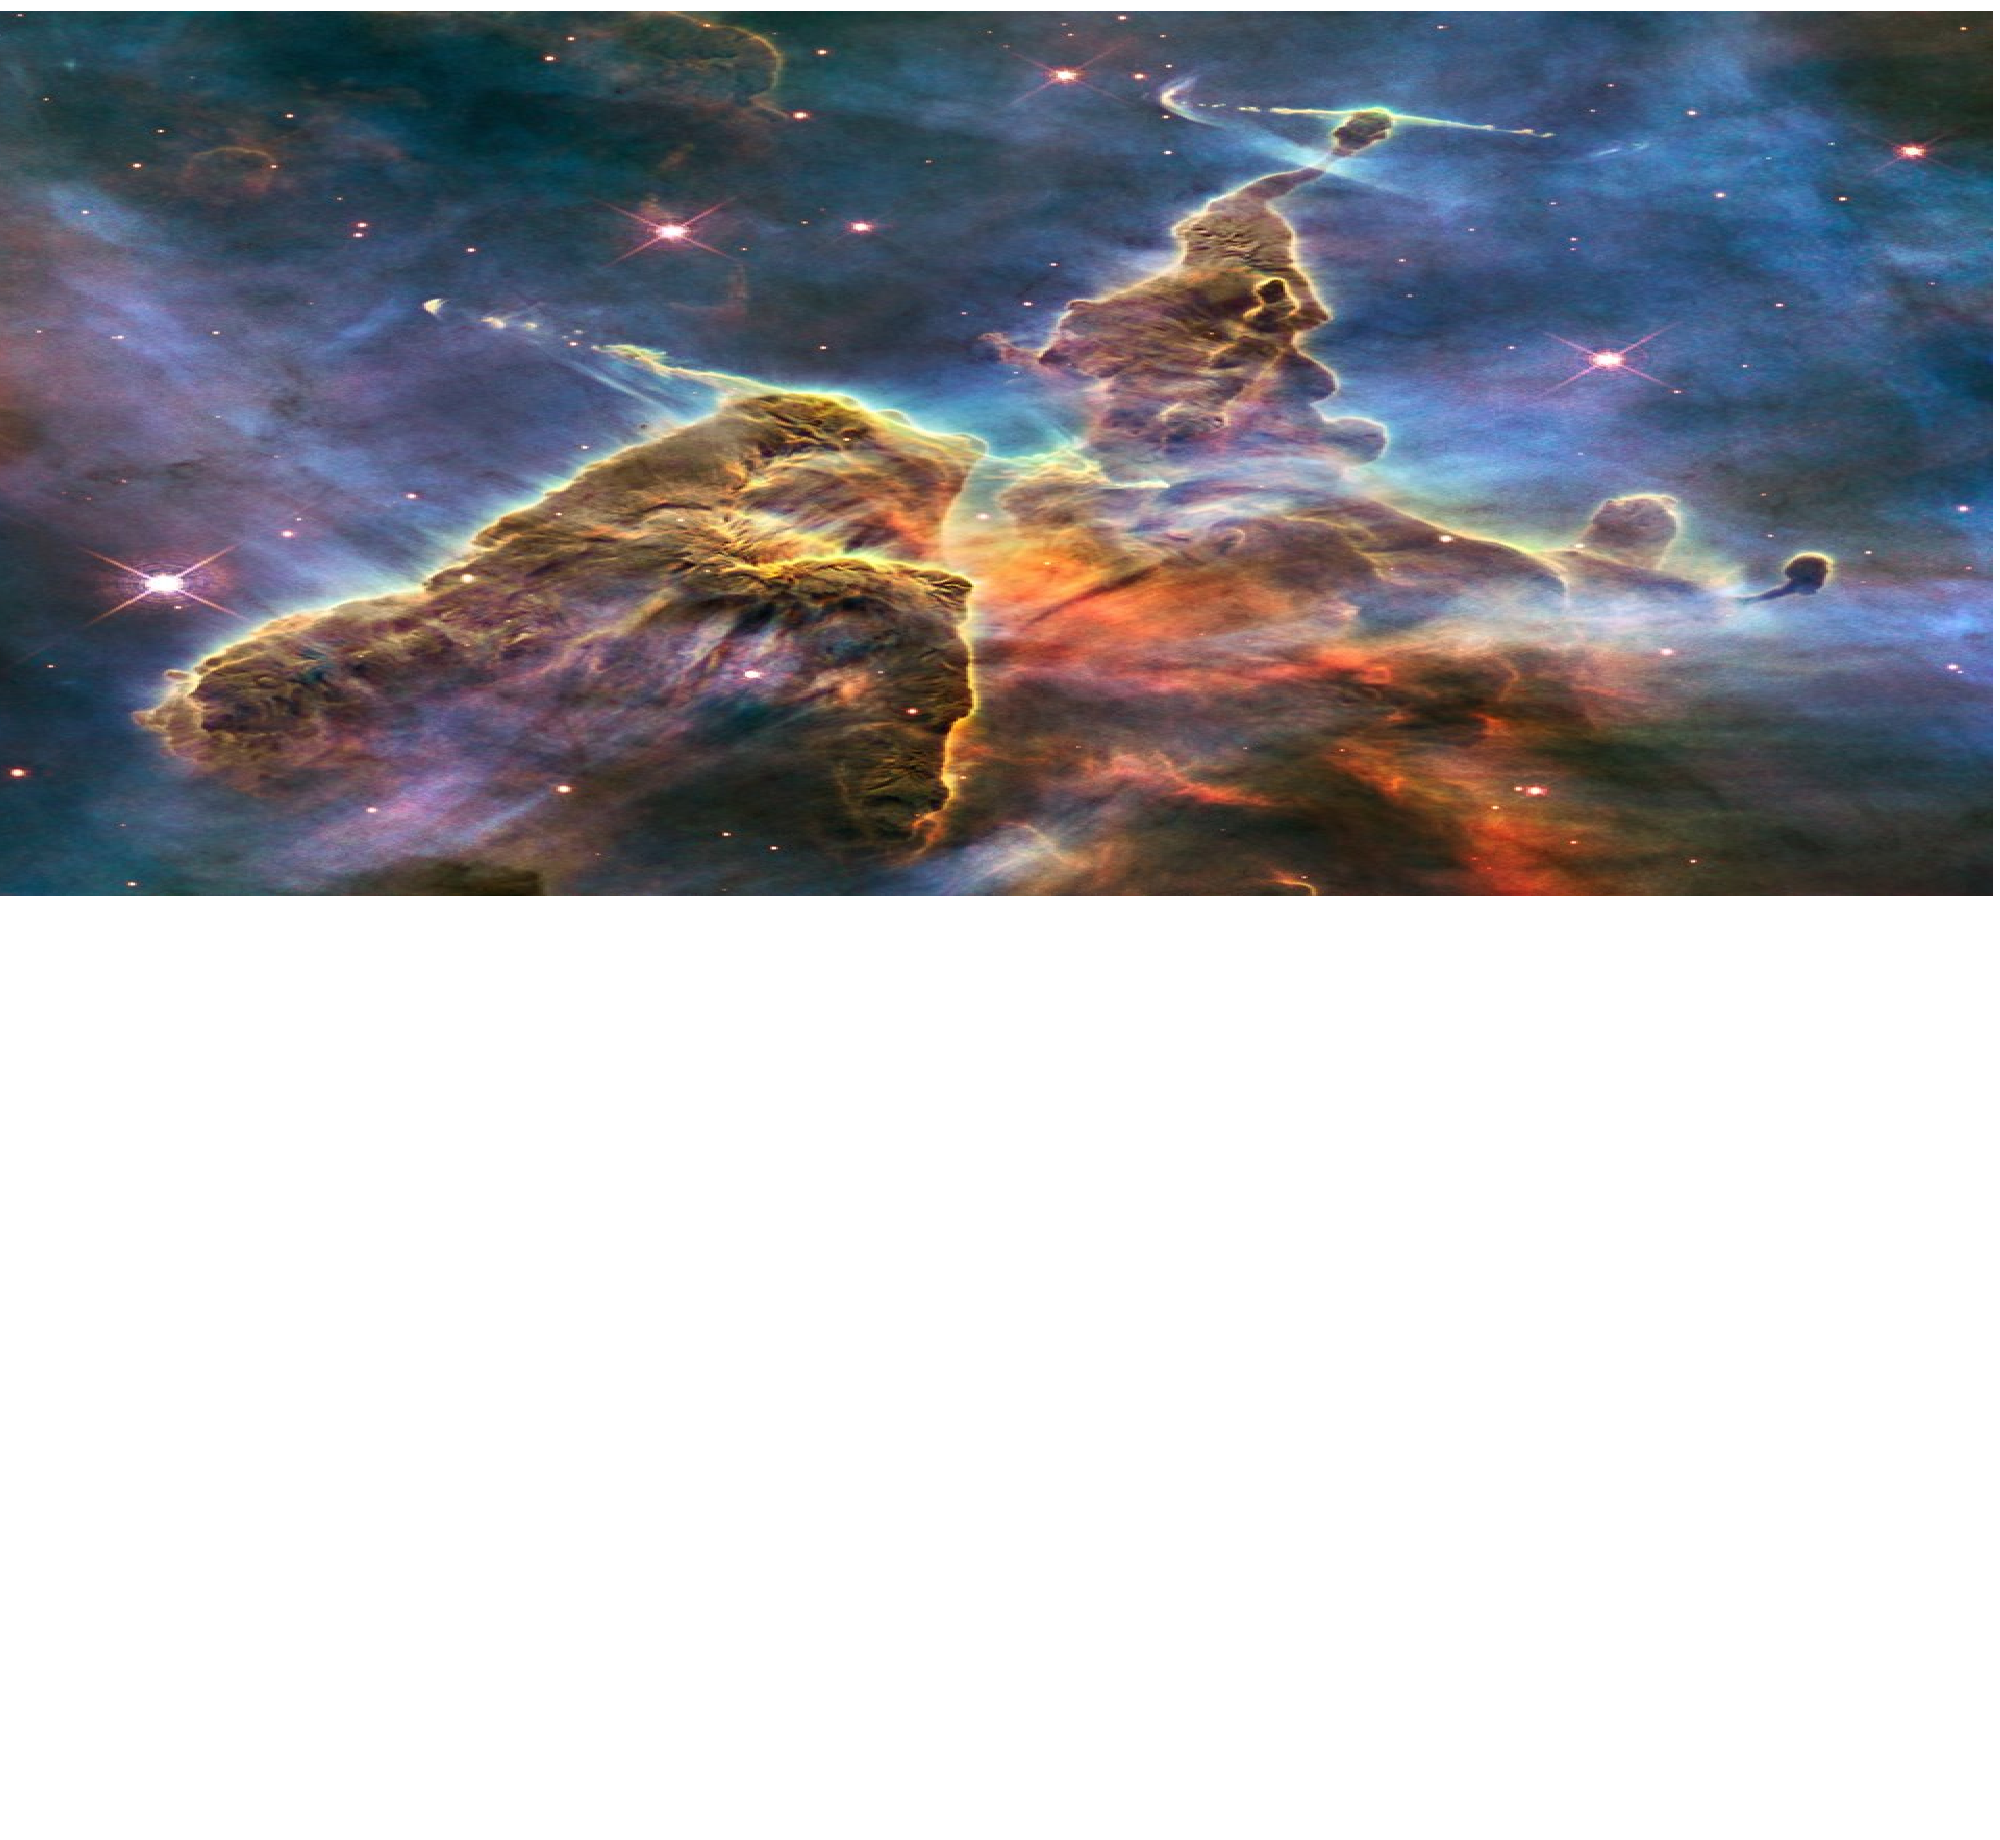
\includegraphics[width=\paperwidth,height=\paperheight]{chapter_head_1.pdf}
%  }%
%}

%----------------------------------------------------------------------------------------
%	HYPERLINKS IN THE DOCUMENTS
%----------------------------------------------------------------------------------------

\usepackage{hyperref}
\hypersetup{backref=true,pagebackref=true,hyperindex=true,colorlinks=false,breaklinks=true,urlcolor= ocre,bookmarks=true,bookmarksopen=false,pdftitle={Title},pdfauthor={Author}}
%\usepackage{bookmark}
%\bookmarksetup{
%open,
%numbered,
%addtohook={%
%\ifnum\bookmarkget{level}=0 % chapter
%\bookmarksetup{bold}%
%\fi
%\ifnum\bookmarkget{level}=-1 % part
%\bookmarksetup{color=ocre,bold}%
%\fi
%}
%}